\documentclass[../MathsNotesBase.tex]{subfiles}

\date{\vspace{-6ex}}

\begin{document}
	\searchableSection{\texorpdfstring{Difference and Differential\\ Equations}{Difference and Differential Equations}}{differential equations, difference equations}
	\bigskip\bigskip
	
	\searchableSubsection{First-order Difference Equations}{difference equations}{
		\bigskip\bigskip
		\note{A \textbf{difference equation} is also known as a \textbf{recurrence equation}.}
		
		\boxeddefinition{Let ${ y_t }$ be the $t$-th value in a sequence (typically $t$ represents time). Then,
			\[ y_t = ay_{t-1} + b, \hspace{20pt} t \geq 1 \]
			is called a \textbf{first-order linear difference equation with constant coefficients}. The value $y_0$ is called an initial condition.\\
			
			A solution to such an equation is an explicit -- or a closed-form (see: \href{https://en.wikipedia.org/wiki/Closed-form_expression}{wikipedia}) -- expression for $y_t$ in terms of $t$ and $y_0$.\\
			
			If ${ b = 0 }$ we have,
			\[ y_t = ay_{t-1} \iff y_t - ay_{t-1} = 0 \]
			which is known as a \textbf{homogeneous} first-order linear difference equation with constant coefficients.
		}
	
		\bigskip
		\labeledProposition{A first-order linear difference equation with constant coefficients of the form ${ y_t = ay_{t-1} + b }$ where ${ a = 1 }$ is a arithmetic progression.
		}{first-order-lin-diff-eqn-const-coeff-1-multiplier-is-arith-prog}
		\begin{proof}
			Let ${ y_t = y_{t-1} + b }$ then,
			\[ y_1 = y_0 + b,\, y_2 = y_1 + b = (y_0 + b) + b = y_0 + 2b,\, y_3 = y_0 + 3b, \dots \]
			so we have ${\bm{ y_t = y_0 + tb }}$. If we describe this as an arithmetic progression we have,
			\[ x_n = a + nd \]
			where the zeroth term $a$ corresponds to $y_0$, the common difference $d$ corresponds to $b$ and, clearly, $t$ and $n$ are both term indices.
		\end{proof}
		
		\bigskip\medskip
		\labeledProposition{A first-order linear difference equation with constant coefficients of the form ${ y_t = ay_{t-1} + b }$ where ${ b = 0 }$ is a geometric progression.}{first-order-lin-diff-eqn-const-coeff-0-const-term-is-geom-prog}
		\begin{proof}
			Let ${ y_t = ay_{t-1} + 0 }$ then,
			\[ y_1 = ay_0,\, y_2 = ay_1 = a(ay_0) = a^2y_0,\, y_3 = a^3y_0, \dots \]
			so we have ${\bm{ y_t = a^ty_0 }}$. If we describe this as a geometric progression we have,
			\[ x_n = ar^n \]
			where the zeroth term $a$ corresponds to $y_0$, the common ratio $r$ corresponds to $a$, and $n$ is the term index corresponding to $t$.
		\end{proof}
	
		\bigskip\medskip
		\labeledProposition{A first-order linear difference equation with constant coefficients of the form ${ y_t = ay_{t-1} + b }$ where ${ a \neq 1 }$ and ${ b \neq 0 }$ has solution
			\begin{align*}
			y_t &= a^t y_0 + b(a^{t-1} + a^{t-2} + \cdots + a + 1) \\
			&= a^t y_0 + b \sum_{i=0}^{t-1} a^i.
			\end{align*}
		}{first-order-lin-diff-eqn-const-coeff-soln-formula}
		\begin{proof}
			\begin{align*}
			y_t &= a y_{t-1} + b \\
			&= a(a y_{t-2} + b) + b = a^2 y_{t-2} + ab + b\\
			&= a^2 (a(y_{t-3} + b)) + ab + b = a^3 y_{t-3} + a^2 b + ab + b \\
			&= a^3 y_{t-3} + b(a^2 + a + 1) \\
			&= a^t y_0 + b(a^{t-1} + \cdots + a + 1).  \qedhere  
			\end{align*}
		\end{proof}
	
		\bigskip\medskip
		\labeledProposition{A first-order linear difference equation with constant coefficients of the form ${ y_t = ay_{t-1} + b }$ where ${ a \neq 1 }$ and ${ b \neq 0 }$ has solution
			\[ y_t = a^t \left(y_0 - \frac{b}{1-a}\right) + \frac{b}{1-a} \]
			where the value
			\[ \frac{b}{1-a} = y^* = a y^* + b \]
			is the \textbf{equilibrium} or \textbf{steady-state} value of the recurrence.
		}{first-order-lin-diff-eqn-const-coeff-soln-formula-wrt-steady-state-value}
		\begin{proof}
			From \autoref{prop:first-order-lin-diff-eqn-const-coeff-soln-formula} we know that the solution to the given recurrence is
			\[ y_t = a^t y_0 + b \sum_{i=0}^{t-1} a^i. \]
			The summation in the second term is the sum of a geometric progression,
			\begin{align*}
			\sum_{i=0}^{t-1} a^i = 1 + a + \cdots + a^{t-1} &= \frac{a^t - 1}{a - 1} \\[8pt]
			&= \frac{a^t}{a - 1} - \frac{1}{a - 1} \\[8pt]
			&= \frac{1}{1 - a} - \frac{a^t}{1 - a}.
			\end{align*}
			So we see that the sum of a geometric progression can be separated into two terms: one term depends on the number of elements in the progression (here $t$), and the other term does not. This is the explanation of the sum of convergent geometric series: if ${ \abs{a} < 1 }$ then, when ${ t \to \infty }$, the $t$-dependent term disappears leaving only the steady-state term.\\
			
			The solution to the recurrence therefore becomes
			\begin{align*}
			y_t &= a^t y_0 + b \left(\frac{1}{1 - a} - \frac{a^t}{1 - a}\right) \\[8pt]
			&= a^t \left(y_0 - \frac{b}{1-a}\right) + \frac{b}{1-a}. \qedhere \\
			\end{align*}
		\end{proof}
	
	
		\biggerskip
		\subsubsection{First-order Linear Difference Equations as Affine Transformations}
		\def\y{\V{y}}
		If we define a vectorized linear difference equation with constant coefficients,
		\[ \y_t = A\y_{t-1} + \b \]
		where $A$ is a matrix, then clearly $\y_t$ is an affine transformation of $\y_{t-1}$.\\
		
		We can linearize this by adding an extra dimension that takes the value 1 like so:
		\[	\begin{bmatrix}
				\y_t\\
				1
			\end{bmatrix} =
			\begin{bmatrix}
				A & \b\\
				0 & 1
	  		\end{bmatrix}
			\begin{bmatrix}
				\y_{t-1}\\
				1
			\end{bmatrix}.
		\]
		
		\bigskip
		A minimal, one-by-one matrix is just a scalar (see: \ref{ex:minimal-linear-transformation}) and a minimal vector can be just a field element (see: \ref{sssection:vectors-as-magnitude-and-direction}) so we can define ${ A = a }$ such that the linearized equation becomes
		\begin{align*}
			\begin{bmatrix}
				y_t\\
				1
			\end{bmatrix} &=
			\begin{bmatrix}
				a & b\\
				0 & 1
			\end{bmatrix}
			\begin{bmatrix}
				y_{t-1}\\
				1
			\end{bmatrix} \\[8pt]
			&=
			\begin{bmatrix}
				a & b\\
				0 & 1
			\end{bmatrix}^t
			\begin{bmatrix}
				y_0\\
				1
			\end{bmatrix}.
		\end{align*}
	
		\bigskip
		\subsubsubsection{Eigenvectors of the Transformation}
		In order to easily take powers of the transformation we find the eigenvectors.\\
		
		Let $M$ be the transformation matrix,
		\[ M = \begin{bmatrix}
				a & b\\
				0 & 1
			\end{bmatrix}
		\]
		
		and, for an eigenvector $\v$,
		\begin{align*}
		&& M \v &= \lambda \v \\
		&\iff & 
		\begin{bmatrix}
		a & b\\
		0 & 1
		\end{bmatrix} \v &= \lambda \v \\[8pt]
		&\iff & \left(
		\begin{bmatrix}
		a & b\\
		0 & 1
		\end{bmatrix} - \lambda I \right) \v &= \0 &\sidecomment{} \\[8pt]
		&\iff &
		\begin{bmatrix}
		a-\lambda & b\\
		0 & 1-\lambda
		\end{bmatrix} \v &= \0 &\sidecomment{} \\[8pt]
		\end{align*}
	
		\begin{align*}
		&& 
		\begin{vmatrix}
		a-\lambda & b\\
		0 & 1-\lambda
		\end{vmatrix} &= 0 \\[8pt]
		&\iff & (a - \lambda)(1 - \lambda) &= 0 &\sidecomment{} \\[8pt]
		&\iff & \lambda \in \{1, a\}.
		\end{align*}
		
		So, for eigenvalue 1:
		\begin{align*}
		&& \begin{bmatrix}
		a-1 & b\\
		0 & 0
		\end{bmatrix} \begin{bmatrix}v_1\\v_2\end{bmatrix} &= \begin{bmatrix}0\\0\end{bmatrix} \\[8pt]
		&\iff & (a - 1)v_1 + b v_2 &= 0 &\sidecomment{} \\[8pt]
		&\iff & (a - 1)v_1 &= -b &\sidecomment{letting ${ v_2 = 1 }$} \\[8pt]
		&\iff & v_1 &= \frac{-b}{a - 1} = \frac{b}{1 - a}\\[8pt]
		&\therefore & \v &= \begin{bmatrix}\frac{b}{1 - a}\\1\end{bmatrix}.
		\end{align*}
		\note{Note that ${ \frac{b}{1 - a} }$ is the steady-state solution of the difference equation.}
		
		For eigenvalue $a$:
		\begin{align*}
		&& \begin{bmatrix}
		0 & b\\
		0 & 1-a
		\end{bmatrix} \begin{bmatrix}v_1\\v_2\end{bmatrix} &= \begin{bmatrix}0\\0\end{bmatrix}  \\[8pt]
		&\iff & v_2 &= 0 &\sidecomment{}\\[8pt]
		&\therefore & \v &= c\begin{bmatrix}1\\0\end{bmatrix} \text{ for } c \in \R{}.
		\end{align*}
		\note{Note that the second component of this vector adds the translation of the affine transformation so this is telling us that if ${ b = 0 }$ then any vector is an eigenvector with eigenvalue $a$. This corresponds to the homogeneous solution.}
		
		\subsubsubsection{Diagonalization}
		\bigskip
		So, if $B$ is the set of two eigenvectors
		\[ \left\{ \begin{bmatrix}\frac{b}{1 - a}\\1\end{bmatrix}, \begin{bmatrix}1\\0\end{bmatrix} \right\} \]
		and we take this as a basis, then the change of basis matrix to this basis is
		\[ P = \inv{[B]} = \inv{\begin{bmatrix}\frac{b}{1 - a} & 1\\1 & 0\end{bmatrix}} 
			= \begin{bmatrix}0 & 1\\1 & \frac{-b}{1 - a}\end{bmatrix} 
		\]
		and the diagonal matrix that represents the transformation with respect to this basis is
		\begin{align*}
		D &= PM\inv{P} \\
		&= \begin{bmatrix}0 & 1\\1 & \frac{-b}{1 - a}\end{bmatrix}
		\begin{bmatrix}
		a & b\\
		0 & 1
		\end{bmatrix}
		\begin{bmatrix}\frac{b}{1 - a} & 1\\1 & 0\end{bmatrix}\\
		&= \begin{bmatrix}0 & 1\\1 & \frac{-b}{1 - a}\end{bmatrix}
		\begin{bmatrix}\frac{b}{1 - a} & a\\1 & 0\end{bmatrix}\\
		&= \begin{bmatrix}1 & 0\\0 & a\end{bmatrix}.
		\end{align*}

		Since $D$ is diagonal we have
		\[ {D}^t = \begin{bmatrix}1 & 0\\0 & a^t\end{bmatrix}. \]
		So, in order to calculate,
		\[ M^t = \begin{bmatrix}
					a & b\\
					0 & 1
				 \end{bmatrix}^t
		 \]
		 we can calculate,
		 \begin{align*}
		 && {D}^t &= (PM\inv{P})^t = PM^t\inv{P} \\
		 &\iff & \inv{P}{D}^tP &= M^t. \\
		 \end{align*}
		 
		 \begin{align*}
		 &\therefore & M^t &= 
		 	\begin{bmatrix}\frac{b}{1 - a} & 1\\1 & 0\end{bmatrix} 
		 	\begin{bmatrix}1 & 0\\0 & a^t\end{bmatrix}
		 	\begin{bmatrix}0 & 1\\1 & \frac{-b}{1 - a}\end{bmatrix} \\
		 &\iff & M^t &= 
		 	\begin{bmatrix}\frac{b}{1 - a} & 1\\1 & 0\end{bmatrix}
		 	\begin{bmatrix}0 & 1\\a^t & \frac{-a^t b}{1 - a}\end{bmatrix} \\
		 &\iff & M^t &= 
		 	\begin{bmatrix}a^t & \frac{b(1 - a^t)}{1 - a}\\0 & 1\end{bmatrix}. \\
		 \end{align*}
		 
		 So, the solution to the first-order linear recurrence is found to be
		 \begin{align*}
		 \begin{bmatrix}
		 y_t\\
		 1
		 \end{bmatrix} &=
		 \begin{bmatrix}
		 a & b\\
		 0 & 1
		 \end{bmatrix}^t
		 \begin{bmatrix}
		 y_0\\
		 1
		 \end{bmatrix} \\
		 &= \begin{bmatrix}a^t & \frac{b(1 - a^t)}{1 - a}\\0 & 1\end{bmatrix} 
		 \begin{bmatrix}
		 y_0\\
		 1
		 \end{bmatrix}
		 \end{align*}
		 
		 so that 
		 \[ y_t = a^t y_0 + \frac{b(1 - a^t)}{1 - a} = a^t\left(y_0 - \frac{b}{1 - a}\right) + \frac{b}{1 - a}. \]
	
		\biggerskip
		\subsubsection{Difference as Rate of change}
		\biggerskip
		\textbf{Geometric progression}: Say we have a first-order linear difference equation with constant coefficients of the form ${ y_t = ay_{t-1} + b }$ where ${ b = 0 }$ so that the terms follow a geometric progression:
		\[ y_1 = ay_0,\, y_2 = a^2y_0,\, y_3 = a^3y_0, \dots \]
		Then the rate of change is
		\[ \frac{\Delta y}{\Delta t} = y_t - y_{t-1} = ay_{t-1} - y_{t-1} = (a - 1)y_{t-1}. \]
		\note{Note that the ratio of consecutive terms remains constant,
			\[ \frac{y_t}{y_{t-1}} = a \]
			which is the "geometric" characteristic of a geometric progression, but the rate of change is proportional to the value.
		}
		The rate of change of the rate of change is, therefore,
		\[ \frac{\Delta^2 y}{\Delta t^2} = (a - 1)\frac{\Delta y_{t-1}}{\Delta t} = (a - 1)\frac{\Delta y}{\Delta t} = (a - 1)^2 y_{t-1}. \]
	
		\bigskip
		\subsubsection{Examples of first-order linear difference equations w/ const. coefficients}
		\begin{exe}
			\item{Let $y_t$ be an account balance after $t$ years and $r$ be the annual interest rate paid on the account. Suppose also, that the interest is compounded $n$ times per year. Then the formula for $y_t$ is,
				\[ y_t = \left(1 + \frac{r}{n}\right)^n y_{t-1} = y_0 \left(1 + \frac{r}{n}\right)^{nt}. \]
				The rate of change per year is,
				\[ \frac{\Delta y}{\Delta t} = y_t - y_{t-1} = \left(1 + \frac{r}{n}\right)^n y_{t-1} - y_{t-1} = \left(\left(1 + \frac{r}{n}\right)^n - 1\right) y_{t-1} \]
				as expected for a geometric progression.\\
				
				If, instead, we let $t$ be continuous we can find the instantaneous rate of change by considering the values for ${ t, t + \Delta t }$,
				\begin{align*}
				\frac{\Delta y}{\Delta t} = \frac{y_{(t + \Delta t)} - y_t}{\Delta t} &=  \frac{y_0 \left(1 + \frac{r}{n}\right)^{n(t + \Delta t)} - y_0 \left(1 + \frac{r}{n}\right)^{nt}}{\Delta t} \\[8pt]
				&= \frac{y_0\left(1 + \frac{r}{n}\right)^{nt}\left(\left(1 + \frac{r}{n}\right)^{n\Delta t} - 1\right)}{\Delta t}
				\end{align*}
				and then letting ${ \Delta t \to 0 }$ to obtain,
				\begin{align*}
				\frac{\dif y}{\dif t} &= \lim_{\Delta t \to 0} \frac{y_0\left(1 + \frac{r}{n}\right)^{nt}\left(\left(1 + \frac{r}{n}\right)^{n\Delta t} - 1\right)}{\Delta t} \\[8pt]
				&= y_0\left(1 + \frac{r}{n}\right)^{nt} \lim_{\Delta t \to 0} \frac{\left(1 + \frac{r}{n}\right)^{n\Delta t} - 1}{\Delta t} &\sidecomment{} \\[8pt]
				&= y_0\left(1 + \frac{r}{n}\right)^{nt} \lim_{\Delta t \to 0} \left[\frac{\dif}{\dif (\Delta t)} \left(1 + \frac{r}{n}\right)^{n\Delta t}\right] &\sidecomment{by L'H\^{o}pital's rule} \\[8pt]
				&= y_0\left(1 + \frac{r}{n}\right)^{nt} \lim_{\Delta t \to 0} \left[n\ln{\left(1 + \frac{r}{n}\right)}\left(1 + \frac{r}{n}\right)^{n\Delta t}\right] &\sidecomment{by \autoref{prop:derivative-of-a-to-power-x-is-ln-a-times-a-to-power-x}} \\[8pt]
				&= ny_0 \ln{\left(1 + \frac{r}{n}\right)} \left(1 + \frac{r}{n}\right)^{nt}
				\end{align*}

				But the question is: How meaningful is this really? If the interest is being compounded only $n$ times per year and these are the only moments when the account balance changes, then change happens at certain discrete moments rather than continuously so is it really meaningful to talk about the instantaneous rate of change? We can recover the discrete-time rate of change per year from this instantaneous one by integrating over a year.\\
				
				Now suppose that $n$, the number of times per year the interest is compounded, goes to infinity. Then (see \ref{sssection:e-to-the-power-x}) we have,
				\[ y_t = y_0 e^{rt}. \]
				For discrete time we have,
				\[ \frac{\Delta y}{\Delta t} = y_0 e^{rt} - y_0 e^{r(t-1)} = y_0 e^{r(t-1)} (e^r - 1) = y_{t-1} (e^r - 1) \]
				which should be no surprise as we still have a geometric progression as
				\[ \frac{y_t}{y_{t-1}} = e^r. \]
				If we now let $t$ be continuous as before then, by a similar logic using L'H\^{o}pital's rule, the instantaneous rate of change obtained is
				\[ \frac{\dif y}{\dif x} = r y_0 e^{rt}. \]
				Note that this is wholly consistent with the discrete time version as we can obtain the discrete time rate of change per year from this instantaneous rate of change by integrating over a year as follows,
				\begin{align*}
				\int_{t-1}^t r y_0 e^{rx} \dif x &= r y_0 \int_{t-1}^t e^{rx} \dif x \\[8pt]
				&= r y_0 \left[\frac{e^{rx}}{r}\right]_{t-1}^t &\sidecomment{} \\[8pt]
				&= y_0 \left[e^{rx}\right]_{t-1}^t &\sidecomment{} \\[8pt]
				&= y_0 (e^{rt} - e^{r(t-1)}) &\sidecomment{} \\[8pt]
				&= y_0  e^{r(t-1)} (e^r - 1). &\sidecomment{}
				\end{align*}
				
				\bigskip
				Now suppose $b$ is deposited at the end of each year so that,
				\begin{align*}
					y_t &= \left(1 + \frac{r}{n}\right)^n y_{t-1} + b \\
					&=  \left(1 + \frac{r}{n}\right)^n \left[ \left(1 + \frac{r}{n}\right)^n y_{t-2} + b \right] + b \\
					&=  \left(1 + \frac{r}{n}\right)^{nt} y_0 + b \sum_{i=0}^{t-1} \left(1 + \frac{r}{n}\right)^{ni}.
				\end{align*}
				But if we, again, let the number of compounds $n$, go to infinity, then,
				\begin{align*}
					y_t &= e^{r} y_{t-1} + b \\
					&=  e^{r} ( e^{r} y_{t-2} + b ) + b \\[6pt]
					&=  y_0 e^{rt} + b \sum_{i=0}^{t-1} e^{ri} \\[6pt]
					&=  y_0 e^{rt} + b \left( \frac{e^{rt} - 1}{e^r - 1} \right) \\[6pt]
					&=  y_0 e^{rt} + b \frac{e^{rt}}{e^r - 1} - b \frac{1}{e^r - 1} \\[6pt]
					&=  \left( y_0 - \frac{b}{1 - e^r} \right) e^{rt} + \frac{b}{1 - e^r}
				\end{align*}	
				where ${ \frac{b}{1 - e^r} }$ is the steady-state value.
			}
		
			\biggerskip
			\item{Let $M_t$ be an account balance at the end of year $t$. Let $Q(t)$ be an amount that is deposited into the account (or withdrawn if the value is negative) one time, at the end of year $t$ and let the interest rate be a fixed rate of $I$. Then,
				\begin{align*}
					M_t &= I M_{t-1} + Q(t) \\
					&= I (I M_{t-2} + Q(t-1)) + Q(t) \\
					&= I (I (I M_{t-3} + Q(t-2)) + Q(t-1)) + Q(t) \\
					&= M_0 I^t + \sum_{i=0}^{t-1} Q(t-i) I^i
				\end{align*}
				and the rate of change is,
				\[ M_t - M_{t-1} = M_0 I^{t-1} (I - 1) + Q(1) I^{t-1} = I^{t-1} (M_0(I - 1) + Q(1)) \]
				which is proportional to $I^{t-1}$.\\
				
				\note{If the interest rate $I$, is also a function of $t$, then -- if we define ${ I(0) = 1 }$ -- we end up with:
					\[ M_t = M_0 \prod_{i=0}^t I(i) + \sum_{i=0}^{t-1} Q(t-i) \prod_{j=0}^i I(i) \]
					which is getting pretty messy. At this point it becomes easier to work with continuous time.
				}
			}
		\end{exe}
	
	}


% ------------------- 	
	
	\pagebreak
	\searchableSubsection{Second-order Difference Equations}{difference equations}{
		\bigskip
		
		\boxeddefinition{A recurrence equation of the form
			\[ y_t = a y_{t-1} + b y_{t-2} + c \]
			where ${ a,b,c \in \R{} }$, is known as a \textbf{second-order linear recurrence with constant coefficients}.
		}
		Following the same approach as with the first-order equations we have,
		\[
			\begin{bmatrix}y_t\\y_{t-1}\\1\end{bmatrix} =
			\begin{bmatrix}
				a & b & c\\
				1 & 0 & 0\\
				0 & 0 & 1
			\end{bmatrix}
			\begin{bmatrix}y_{t-1}\\y_{t-2}\\1\end{bmatrix}.
		\]
		Determining eigenvalues we get,
		\begin{align*}
		&&	\begin{vmatrix}
				a-\lambda & b & c\\
				1 & -\lambda & 0\\
				0 & 0 & 1-\lambda
			\end{vmatrix} &= 0 \\[3pt]
		&\iff & (1-\lambda)((-\lambda)(a-\lambda) - b) &= 0 &\sidecomment{} \\[3pt]
		&\therefore & \lambda \in \left\{ 1, \frac{a + \sqrt{a^2 + 4b}}{2}, \frac{a - \sqrt{a^2 + 4b}}{2} \right\}.
		\end{align*}
		
		Due to the translation represented by the lone 1 in the final row of the matrix, there will always be the eigenvalue 1. This corresponds to the steady state value which may be thought of as the eigenvector of the translation. The other two eigenvalues are the eigenvectors of the linear transformation part of the affine transformation. The block structure is as follows.
		
		\begin{align*}
		&&	\begin{bmatrix}
			\begin{bmatrix}a & b\\1 & 0\end{bmatrix} & \begin{bmatrix}c\\0\end{bmatrix} \\
			\begin{bmatrix}0 & 0\end{bmatrix} & \begin{bmatrix}1\end{bmatrix}	
		\end{bmatrix}
		\begin{bmatrix}y_{t-1}\\y_{t-2}\\1\end{bmatrix} &= 
		\begin{bmatrix}a & b\\1 & 0\end{bmatrix}\begin{bmatrix}y_{t-1}\\y_{t-2}\end{bmatrix} +
		\begin{bmatrix}c\\0\end{bmatrix} \\
		&&  &= A\V{y} + \V{t}. \\
		\end{align*}
		
		\subsubsubsection{Steady-state value}
		Considering the case of the eigenvalue ${ \lambda = 1 }$ we have,
		\[
			\begin{bmatrix}
				a-1 &  b & c \\
				1   & -1 & 0 \\
				0   &  0 & 0
			\end{bmatrix}
			\begin{bmatrix}y_{t-1}\\y_{t-2}\\1\end{bmatrix} =
			\begin{bmatrix}0\\0\\0\end{bmatrix}. 
	    \]
	    So, to find the nullspace of the matrix we can find the row-reduced echelon form,
	    \begin{align*}
	    && 	\begin{bmatrix}
		    	a-1 &  b & c \\
		    	1   & -1 & 0 \\
		    	0   &  0 & 0	
		    \end{bmatrix} &\leadsto
		    \begin{bmatrix}
			    1 &  \frac{b}{a-1} & \frac{c}{a-1} \\
			    1   & -1 & 0 \\
			    0   &  0 & 0	
		    \end{bmatrix} \\[4pt]
	    &\leadsto & 
		    \begin{bmatrix}
			    1 &  \frac{b}{a-1} & \frac{c}{a-1} \\
			    0  & -1-\frac{b}{a-1} & -\frac{c}{a-1} \\
			    0   &  0 & 0	
		    \end{bmatrix} &\leadsto 
		    \begin{bmatrix}
			    1 &  \frac{b}{a-1} & \frac{c}{a-1} \\
			    0   & 1 & \frac{c}{a+b-1} \\
			    0   &  0 & 0	
		    \end{bmatrix}  \\[4pt]
		&\leadsto &
			\begin{bmatrix}
				1 & 0 & \frac{c}{a+b-1} \\
				0 & 1 & \frac{c}{a+b-1} \\
				0 & 0 & 0	
			\end{bmatrix}
	    \end{align*}
	    where the last step is because
	  	\begin{align*}
	  	\frac{c}{a-1} - \left(\frac{b}{a-1}\right)\frac{c}{a+b-1} &= \frac{c}{a-1}\left(1 - \frac{b}{a+b-1}\right) \\
	  	&= \frac{c}{a-1}\left(\frac{a-1}{a+b-1}\right). \\
	  	\end{align*} 
	  	
	  	So the nullspace is
	  	\[ t\begin{bmatrix}
		  		\frac{-c}{a+b-1} \\[4pt] \frac{-c}{a+b-1} \\[4pt] 1	
		  	\end{bmatrix} 
		\]
		for any ${ t \in \R{} }$ and the steady-state value is
		\[ \frac{-c}{a+b-1}. \]
		\note{This is also sometimes referred to as a \textbf{particular solution of the non-homogeneous equation}.}
		
		\bigskip
		\subsubsubsection{Eigenvalues of the linear transformation}
		Let the discriminant ${ d = \sqrt{a^2 + 4b} }$. Then the eigenvalues of the linear transformation are
		\[ \frac{a + d}{2} \eqand \frac{a - d}{2}. \]
		In the case of the eigenvalue ${ \frac{a + d}{2} }$ we have,
		\[
		\begin{bmatrix}
			\frac{a - d}{2} &  b & c \\
			1   & -(\frac{a + d}{2}) & 0 \\
			0   &  0 & 1-(\frac{a + d}{2})
		\end{bmatrix}
		\begin{bmatrix}y_{t-1}\\y_{t-2}\\1\end{bmatrix} =
		\begin{bmatrix}0\\0\\0\end{bmatrix}. 
		\]
		Again using row reduction to find the nullspace:
		\begin{align*}
		&& 	\begin{bmatrix}
			\frac{a - d}{2} &  b & c \\[4pt]
			1   & -(\frac{a + d}{2}) & 0 \\[4pt]
			0   &  0 & 1-(\frac{a + d}{2})	
		\end{bmatrix} &\leadsto
		\begin{bmatrix}
			1   & -(\frac{a + d}{2}) & \frac{2c}{a - d} \\[4pt]
			1   & -(\frac{a + d}{2}) & 0 \\[4pt]
			0   &  0 & 1-(\frac{a + d}{2})
		\end{bmatrix} &\sidecomment{using ${ \frac{2b}{a - d}\frac{a + d}{a + d} = -(\frac{a + d}{2}) }$}\\[4pt]
		&\leadsto & 
		\begin{bmatrix}
			1   & -(\frac{a + d}{2}) & \frac{2c}{a - d} \\[4pt]
			0   &  0 & \frac{-2c}{a - d} \\[4pt]
			0   &  0 & 1-(\frac{a + d}{2})	
		\end{bmatrix} &\leadsto 
		\begin{bmatrix}
			1   & -(\frac{a + d}{2}) & \frac{2c}{a - d} \\[4pt]
			0   &  0 & 1 \\[4pt]
			0   &  0 & 1	
		\end{bmatrix}  \\[4pt]
		&\leadsto &
		\begin{bmatrix}
			1   & -(\frac{a + d}{2}) & 0 \\[4pt]
			0   &  0 & 1 \\[4pt]
			0   &  0 & 0
		\end{bmatrix}
		\end{align*}
		
		So the nullspace is
		\[ t\begin{bmatrix}
				\frac{a + d}{2} \\[4pt] 1 \\[4pt] 0	
			\end{bmatrix} 
		\]
		for any ${ t \in \R{} }$ and the value
		\[ \frac{a + d}{2} = \frac{a + \sqrt{a^2 + 4b}}{2} \]
		is the solution to the homogeneous equation corresponding to the eigenvalue ${ (a+d)/2 }$. It's also not hard to see that the other eigenvalue ${ (a-d)/2 }$ results in the solution to the homogeneous equation
		\[ \frac{a - d}{2} = \frac{a - \sqrt{a^2 + 4b}}{2}. \]
		
		\medskip
		\note{Another common way of finding these solutions in this case is to form what is known as the \textbf{auxiliary equation} as:
			\begin{align*}
			&& y_t - a y_{t-1} - b y_{t-2} &= 0 \\
			&\leadsto & m^t - a m^{t-1} - b m^{t-2} &= 0 &\sidecomment{for some ${ m \neq 0 \in \R{} }$} \\
			&\iff & m^{t-2}(m^2 - a m - b) &= 0 &\sidecomment{} \\
			&\iff & m^2 - a m - b &= 0. &\sidecomment{since ${ m \neq 0 }$} \\
			\end{align*} 
		Note that this is the characteristic polynomial of the linear transformation part of the matrix:
		\[ (-\lambda)(a-\lambda) - b = \lambda^2 - a \lambda - b. \]}
	
		\medskip
		In this case, determining the final equation for ${ y_t }$ using matrix powers results in a very complex matrix and formula which is only reasonably performed on a computer. But we can infer that the formula will involve the eigenvalues of the linear transformation, raised to the power $t$, and the steady-state value,
		\[ y_t = C_1 \frac{(a+d)^t}{2^t} + C_2 \frac{(a-d)^t}{2^t} + \frac{c}{a+b-1}. \]
		
		Then we can use the initial values to solve for the constants ${ C_1, C_2 }$,
		\[ y_0 = C_1 + C_2 + \frac{c}{a+b-1} \eqand y_1 = C_1 \frac{a+d}{2} + C_2 \frac{a-d}{2} + \frac{c}{a+b-1}. \]
		
		The values 
		\[ \frac{a+d}{2} = \frac{a + \sqrt{a^2 + 4b}}{2} \eqand \frac{a-d}{2} = \frac{a - \sqrt{a^2 + 4b}}{2} \]
		may be two distinct real values, one real value (if ${ a^2 + 4b = 0 }$) or two distinct complex values (if ${ a^2 + 4b < 0 }$).
		
		\paragraph{In the case of one real value:} the formula becomes,
		\[ y_t = (C_1 + C_2 t) \frac{(a+d)^t}{2^t} + \frac{c}{a+b-1}. \]
		The explanation of this appears to be that the matrix ${ A - \lambda I }$ has cyclic order 2. \TODO{? eh?}
		
		\paragraph{In the case of two complex values:} expressing the eigenvalues in exponential form we have,
		\begin{align*}
		\frac{a}{2} \pm \frac{\sqrt{-a^2 - 4b}}{2} i &= \sqrt{ \frac{a^2}{4} + \frac{-a^2 - 4b}{4} }\, \exp\left(i\arctan{\pm\frac{\sqrt{-a^2 - 4b}}{a}}\right) \\[4pt]
		&= \sqrt{-b}\, \exp\left(i\arctan{\pm\sqrt{-1 - \frac{4b}{a^2}}}\right).
		\end{align*}
		Let 
		\[ \theta = \arctan{\sqrt{-1 - \frac{4b}{a^2}}} \eqand -\theta = \arctan{-\sqrt{-1 - \frac{4b}{a^2}}}. \]
		Then the eigenvalues raised to the power of $t$ are:
		\[ (\sqrt{-b})^t\, e^{i \theta t} \eqand (\sqrt{-b})^t\, e^{-i \theta t} \]
		which means that the formula becomes,
		\begin{align*}
		y_t &= C_1(\sqrt{-b})^t\, (\cos(\theta t) + i \sin(\theta t))\\[8pt]
			&\hspace{18pt} +  C_2(\sqrt{-b})^t\, (\cos(-\theta t) + i \sin(-\theta t)) \\[8pt]
			&\hspace{18pt} +  \frac{c}{a+b-1} \\[8pt]
		&= C_1(\sqrt{-b})^t\, (\cos(\theta t) + i \sin(\theta t))\\[8pt]
			&\hspace{18pt} +  C_2(\sqrt{-b})^t\, (\cos(\theta t) - i \sin(\theta t)) \\[8pt]
			&\hspace{18pt} +  \frac{c}{a+b-1} &\sidecomment{} \\[8pt]
		&= (\sqrt{-b})^t\, (C_1 + C_2)\cos(\theta t) \\[8pt]
			&\hspace{18pt} + i (\sqrt{-b})^t\, (C_1 - C_2) \sin(\theta t) \\[8pt]
			&\hspace{18pt} +  \frac{c}{a+b-1} &\sidecomment{} \\[8pt]
		&= (\sqrt{-b})^t\, (C_3\cos(\theta t) + i C_4 \sin(\theta t)) +  \frac{c}{a+b-1}.
		\end{align*}
		
		But, since we are looking for real-valued solutions and any linear combination of the homogeneous solutions is also a homogeneous solution, we can generate other, real-valued homogeneous solutions from linear combinations of these ones. In fact, we can just divide the imaginary solution by $i$ so that our real-valued solution is:
		\[ (\sqrt{-b})^t\, (C_3\cos(\theta t) + C_4 \sin(\theta t)) +  \frac{c}{a+b-1}. \]
		\TODO{eh? if divide by $i$ then the real part will be divided by $i$ also}
		
	}




% ----------------------------------


	\pagebreak
	\searchableSubsection{Markov Chains}{difference equations}{
		\biggerskip
		
		\subsubsection{Markov Matrices (a.k.a. Stochastic Matrices)}
		\note{This section taken from \href{http://people.math.harvard.edu/~knill/teaching/math19b_2011/handouts/lecture33.pdf}{Harvard}.}
		
		\boxeddefinition{An \( n \times n \) matrix is called a \textbf{Markov} or \textbf{Stochastic} matrix if all entries are nonnegative and the sum of each column vector is equal to 1.}
		
		The matrix
		\[
		A=\left[\begin{array}{ll}
		1 / 2 & 1 / 3 \\
		1 / 2 & 2 / 3
		\end{array}\right]
		\]
		is a Markov matrix.\\
		
		\note{Many authors write the transpose of the matrix and apply the matrix to the right of a row vector.}
		
		Let's call a vector with nonnegative entries \( p_{k} \) for which all the \( p_{k} \) add up to 1 a stochastic vector. For a stochastic matrix, every column is a stochastic vector.
		
		\labeledTheorem{If \( p \) is a stochastic vector and \( A \) is a stochastic matrix, then \( A p \) is a stochastic vector.}{stochastic-vector-times-stochastic-matrix-is-stochastic}
		\begin{proof}
			Let \( v_{1}, \ldots, v_{n} \) be the column vectors of \( A . \) Then
			\[
			A p=\left[\begin{array}{c}
			p_{1} \\
			p_{2} \\
			\cdots \\
			p_{n}
			\end{array}\right]=p_{1} v_{1}+\ldots+v_{n} v_{n}
			\]
			If we sum this up we get \( p_{1}+p_{2}+\ldots+p_{n}=1 \).
		\end{proof}
	
		\biggerskip
		\labeledTheorem{A Markov matrix \( A \) always has an eigenvalue \( 1 . \) All other eigenvalues are in absolute value smaller or equal to \( 1 . \)}{stochastic-matrix-eigenvalues-are-1-and-absolutely-less-than-1}
		\begin{proof}
			For the transpose matrix \( A^{T}, \) the sum of the row vectors is equal to \( 1 . \) The matrix \( A^{T} \) therefore has the eigenvector
			\[
			\left[\begin{array}{c}
			1 \\
			1 \\
			\cdots \\
			1
			\end{array}\right].
			\]
			Because \( A \) and \( A^{T} \) have the same determinant, also \( A-\lambda I_{n} \) and \( A^{T}-\lambda I_{n} \) have the same determinant so that the eigenvalues of \( A \) and \( A^{T} \) are the same (\TODO{we can reference the proof that a matrix is similar to its transpose but does this explanation also make sense?}). With \( A^{T} \) having an eigenvalue 1 also \( A \) has an eigenvalue 1 Assume now that \( v \) is an eigenvector with an eigenvalue \( |\lambda|>1 . \) Then \( A^{n} v=|\lambda|^{n} v \) has exponentially growing length for \( n \rightarrow \infty . \) This implies that there is for large \( n \) one coefficient \( \left[A^{n}\right]_{i j} \) which is larger than \( 1 . \) But \( A^{n} \) is a stochastic matrix (see homework) and has all entries \( \leq 1 . \) The assumption of an eigenvalue larger than 1 can not be valid.
		\end{proof}
	
		\note{For there to be a long-term distribution of the markov chain it is necessary that the eigenvalue 1 in the markov matrix have multiplicity 1. Otherwise, there may be more than one eigenvector corresponding with eigenvalue 1 or the matrix may not be diagonalizable. In the case that it is diagonalizable, there will only be one eigenvector with eigenvalue 1 that is also a distribution vector (stochastic vector).}
	}


% ----------------------------------


	\pagebreak
	\searchableSubsection{Differential Equations}{differential equations}{
		\biggerskip
		
		Differential equations are most often used to describe the evolving state of dynamical systems -- that is, systems whose future state is a function of its current state. Therefore, that portion of the future state that is dependent on the previous state is compounded in a similar fashion to compound interest. For this reason, the solutions to differential equations typically involve the exponential function.\\
		
		\subsubsection{Types of Differential Equations}
		
		\boxeddefinition{A \textbf{differential equation} -- that is, a single equation as opposed to a system of equations -- is an equation that relates a single dependent variable's derivatives to each other and may or may not explicitly include the independent variable. A common convention is for the dependent variable to be $y$ and the independent variable to be $t$ -- reflecting the fact that it is often modelling time -- but $x$ is often used also.}
		
		\boxeddefinition{A differential equation that does not explicitly include the independent variable is known as an \textbf{autonomous} equation. It represents a time-invariant system if the independent variable is viewed as time. So, if ${ y(t) = g(t) }$ is a solution then ${ y(t) = g(t+c) }$, for constant $c$, is also a solution.}
		
		\boxeddefinition{A \textbf{first-order} differential equation is an equation in which only derivatives upto and including the first derivative of the dependent variable appear. That's to say, an equation that relates the dependent variable to its first derivative and, potentially, to the independent variable.}
		
		\boxeddefinition{Similarly, a \textbf{second-order} differential equation relates the dependent variable to both its first and second derivatives as well as, potentially, to the independent variable. Higher-order differential equations also exist -- but are less common -- with the order being given by the highest derivative present in the equation.}
		
		\boxeddefinition{A \textbf{linear} differential equation is an equation containing only degree-one monomial terms in the derivatives of the dependent variable. So, the equation is linear in the derivatives of the dependent variable although it may also contain any function of the independent variable.
		}
	
		\boxeddefinition{A \textbf{nonlinear} differential equation is an equation that contains nonlinear terms of the derivatives of the dependent variable.}
		
		\boxeddefinition{A \textbf{separable} first-order equation is one where the first-derivative of the dependent variable may be expressed as a single term. That's to say, we can put the equation in the form,
			\[ \dod{y}{t} = f(t)g(y). \]
		}
		\note{Note that the definition of a separable equations means that -- if $A,B,C,D$ are constants -- the following equation is separable,
			\[ \dod{y}{t} = ABt^2y^2 + ADt^2 + BCy^2 + CD \]
			because it can be factorized into,
			\[ \dod{y}{t} = (At^2 + C)(By^2 + D) = f(t)g(y). \]
		}
		
		\boxeddefinition{A \textbf{partial} differential equation is a differential equation that includes at least one partial derivative. Otherwise, a differential equation is known as an \textbf{ordinary} differential equation. The two terms are frequently abbreviated to ODE and PDE.}
		
		
		\bigskip
		\subsubsection{Solutions}
		\boxeddefinition{A \textbf{solution} to a differential equation -- also called a \textbf{general solution} -- is a set of functions that share the relation expressed in the differential equation.}%
		\note{This is similar to the solution to an indefinite integral being a set of antiderivatives. However, an indefinite integral determines an antiderivative upto an additive constant but the general solution of a differential equation may only determine a function upto a multiplicative constant.}
		
		\medskip
		\boxeddefinition{A \textbf{solution to the initial value problem} of a differential equation is a specific function where the initial value has determined a particular member of the set of functions in the general solution. That's to say, it is a function that \textbf{both} exhibits the relation in the differential equation and satisfies the initial condition(s) of the initial value problem.}
		
		
		\note{A general solution of a differential equation defines a direction field where at every co-ordinate -- $(x,y)$ or $(t,y)$ -- the gradient is defined by the equation ${ \tod{y}{t} = f(t,y) }$. The solution to an IVP is a path through this direction field beginning at a point $(t_0, y_0)$ representing the initial conditions.}
		\begin{figure}[h!]
			\caption{The direction field of ${ y' = \sin(y) }$. The field contains steady-states at ${ y = 0,\pi,\frac{pi}{2} }$.}\label{fig:Dy_eq_sin_y}
			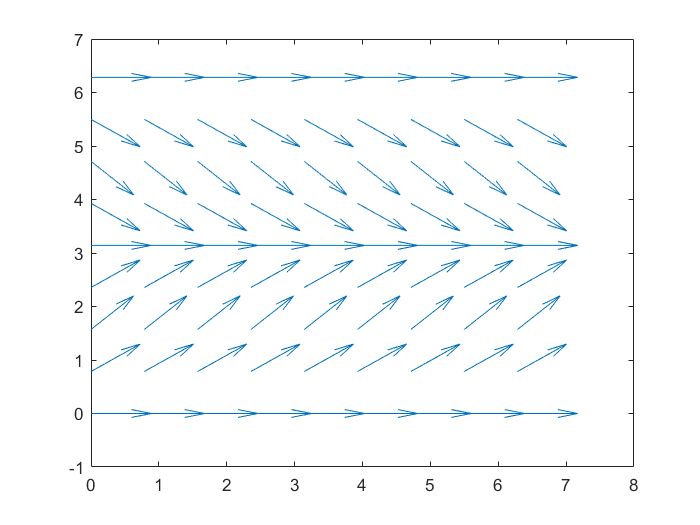
\includegraphics[width=\linewidth]{\resourceDir/img/Dy_eq_sin_y.png}
		\end{figure}
		\biggerskip
		
		
		\biggerskip
		\subsubsection{Equilibrium Points / Steady-states}
		
		\boxeddefinition{A \textbf{steady-state} solution is an IVP solution that is constant across all values of the independent variable. Therefore, the initial conditions of the IVP must be this constant value.\\
		For example, if ${ y(t) = C }$ for some constant $C$, is a steady-state solution then, for the initial condition ${ y(t_0) = C }$, the constant function ${ y(t) = C }$ is a solution to the IVP. Since this function is constant for all values of $t$, the derivative ${ \tod{y}{t} = 0 }$ also at all values of $t$.}
		
		\note{Although a function ${ y(t) = C }$ is only a solution to the IVP ${ y(t_0) = C }$ other solutions satisfying other initial conditions may converge to the value $C$. In this way, the steady-state may be the long-term behaviour of IVP solutions from a whole set of initial conditions.}
		
		\note{If we take the general form of a first-order differential equation
				\[ \dod{y}{t} = f(t)g(y) + h(t), \]
			then, for some value of the function $y_s$ to be a steady-state solution we need, for all $t$,
				\begin{align*}
					&& \dod{y}{t} = f(t)g(y_s) + h(t) &= 0 \\
					&\iff &  g(y_s) &= -\frac{h(t)}{f(t)}.
				\end{align*}
			For example, the equation ${ y' = \frac{4t}{y} - 2t }$ has a steady-state at ${ y = 2 }$.
		}
		
		\medskip
		\boxeddefinition{A steady-state is called \textbf{stable} if the set of initial conditions that converge to it is greater than its value alone. In other words, if ${ y(t) = C }$ is a steady-state, then it is stable if the set of all initial values of the function ${ y_0 = y(t_0) }$ whose IVP solutions converge to it, 
			\[ S = \setc{y_0}{y(t_0) = y_0 \implies \lim_{t \to \infty} y(t) = C} \]
		is a proper superset of $\set{C}$ -- i.e. ${ \set{C} \subsetneq S }$.\\
		
		Conversely, a steady-state is called \textbf{unstable} if the set of initial conditions that converge to it is only the value itself. That's to say,
			\[ S = \set{C}. \]
			
		A steady-state can also be \textbf{semi-stable} if it is stable from one side and unstable from the other.
		}
	
		\note{Stable steady-states happen when greater values of the function decrease to the steady-state value and lesser values of the function increase to the steady-state value. An \textbf{unstable} steady-state, conversely, is one where values of the function that are a little lesser and greater move away from the steady-state value. The states of real-world systems modelled by these unstable steady-states may sometimes not, in practice, be referred to as equilibria due to their instability.
		}
	
		\bigskip
		\subsubsubsection{Examples of types of steady-state}
		\begin{exe}
			\ex{A ball rolling into a dip in the ground stays there whereas a ball at the top of a hump in the ground will likely roll off. If a dip in the ground is described by the curve ${ y = x^2 }$ so that the stable equilibrium is at ${ x = 0 }$ then, if the ball is pushed and rolls up the hill on the right side, the potential energy gained is proportional to $x^2$ and the tendency to return to the equilibrium is dependent on the rate at which the potential energy is released as the ball rolls back to the bottom, which is ${ \tod{x^2}{x} = 2x }$. Since this is acting to reduce the value of the displacement $x$ its sign is negative so $-2x$. Clearly the converse is the situation for a hump in the ground. So, in this model, the dip in the ground has a gradient field with a maximum at the equilibrium (similar to the curve of ${ y = -x^2 }$) while the hump in the ground has a gradient field with a minimum at the equilibrium (similar to the curve of ${ y = x^2 }$).
			}
			\medskip
			\ex{The equation ${ y' = \sin(y) }$ in figure \ref{fig:Dy_eq_sin_y} shows a stable equilibrium at ${ y = \pi }$ and unstable equilibria at ${ y = 0, 2\pi }$. This is because ${ \tpd{}{y} \sin(y) = \cos(y) }$ which is negative around ${ y = \pi }$ -- so this is a maximum and therefore, stable -- and positive around the values ${ y = 0, 2\pi }$ -- so these are minimums and therefore, unstable.
			}
			\medskip
			\ex{Another example: The equation ${ y' = \frac{4t}{y} - 2t }$ has a \textbf{stable} steady-state at ${ y = 2 }$ for positive $t$ but at the same $y$-value the steady-state is unstable for negative values of $t$. This is because ${ \tpd{}{y}\left(\frac{4t}{y} - 2t\right) = -\frac{4t}{y^2} = -t }$ at ${ y = 2 }$ which means that the steady-state is a maximum and stable for positive $t$ and a minimum and unstable for negative $t$.
				\note{Note that, if $t$ is modelling time, negative values of $t$ may not be meaningful.}
			}
			\medskip
			\ex{The equation ${ y' = y^2 }$ has a semi-stable steady-state at ${ y = 0 }$: solution curves below it converge to it, but those above it diverge. Why? At ${ y = 0 }$ we have ${ \tpd{}{y} y^2 = 2y = 0 }$ so this is an inflection point. We look at before and after and see that both have positive values of the gradient $y'$.
			}\label{ex:Dy-eq-y-squared}
			\medskip
			\ex{A corner case: The equation ${ y' = 2\sqrt{y} }$. This has a steady-state at ${ y = 0 }$ which is unstable from above because ${ \tpd{}{y} (2\sqrt{y}) = \frac{1}{\sqrt{y}} }$ is positive for positive $y$ so this is a minimum when viewed from above. But the partial derivative has an infinite discontinuity as ${ y = 0 }$ and doesn't exist as a real number for negative $y$. Likewise the gradient $y'$ is not a real number for negative $y$ and so is undefined in this situation. 
			}\label{ex:Dy-eq-2-sqrt-y}
		\end{exe}
	}


% ----------------------------------


	\pagebreak
	\searchableSubsection{First-order Linear ODEs}{differential equations}{
		\bigskip\bigskip
		
		\subsubsubsection{The form ${ \frac{\dif y}{\dif x} = f(x)y }$}
		The most simple form has a single $y$-term whose coefficient may be a function of $x$. This form is separable as,
		\begin{align*}
		&& \frac{\dif y}{\dif x} &= f(x)y \\[8pt]
		&\iff & \frac{1}{y} \frac{\dif y}{\dif x} &= f(x) &\sidecomment{} \\[8pt]
		&\iff & \int \frac{1}{y} \frac{\dif y}{\dif x} \dif x &= \int f(x) \dif x &\sidecomment{} \\[8pt]
		&\iff & \ln \abs{y} &= F(x) + c &\sidecomment{${ y \neq 0 }$, $F$ is an antiderivative of $f$} \\[8pt]
		&\iff & \abs{y} &= e^{F(x)}\cdot e^c &\sidecomment{} \\[8pt]
		&\iff & y &= ke^{F(x)} &\sidecomment{${ k \in \R{}. }$}
		\end{align*}
		Check solution:
		\[ \frac{\dif y}{\dif x} = f(x)ke^{F(x)} = f(x)y. \]
		\note{Note that the solution has the form,
			\[ y = ke^{F(x)} \]
			where $F(x)$ is an antiderivative of $f(x)$, the coefficient of $y$ in the original differential equation. Since the antiderivative is unique upto a constant factor, the other possible antiderivatives are achieved by the value of the coefficient $k$ because,
			\[ e^{F(x) + c} = e^{F(x)}\cdot e^c = ke^{F(x)}. \]
		}
	
		\subsubsubsection{I.V.P. Solution}
		If we have an initial value for the function -- say ${ y(t_0) = y_0 }$ -- then we need 
			\[ y(t_0) = y_0 = y_0 (1) = y_0 e^0 = y_0 e^{\int_{t_0}^t f(x) \dif x}. \]
		That's to say, with the addition of an initial value, the general solution,
			\[ y(t) = e^{\int f(t) \dif t} = k e^{F(t)} \]
		becomes a complete solution,
			\[ y(t) = y_0 e^{\int_{t_0}^t f(x) \dif x}. \]
		We can see the equivalence by setting the constant $k$ in the general solution to ${ y_0 / e^{F(t_0)} }$,
			\[ y(t) = \frac{y_0}{e^{F(t_0)}} e^{F(t)} = y_0 \frac{ e^{F(t)} }{ e^{F(t_0)} } = y_0 e^{(F(t) - F(t_0))} = y_0 e^{\int_{t_0}^t f(x) \dif x}. \]
	
		\sep
		\subsubsubsection{Separable Equations}
		Any equation of the form ${ \frac{\dif y}{\dif x} = f(x)y }$ is separable into the form,
		\[ f(x) \dif x = g(y) \dif y \]
		and can then be solved by integrating both sides. As a result, the solution moves on level sets of ${ \int f(x) \dif x - \int g(y) \dif y }$. This value, then, is invariant (i.e. constant) across all solutions and so, tends to represent a conserved quantity in physical systems. Therefore, these type of equations, when modelling physical systems, could be described as modelling closed systems with no external influence.
	
		\biggerskip
		\subsubsubsection{Examples}
		\begin{exe}
			\ex{Say we have an IVP (Initial Value Problem) such that our independent variable is $t$ beginning at 0, with ${ y(0) = y_0 }$, and
				\[ \frac{\dif y}{\dif t} = f(t) y.  \]
				Then if we look at what happens at integral intervals of $t$ we can see that:
				\begin{align*}
					y(0) &= y_0 \\
					y(1) &= y_0 e^{\int_0^1 f(t) dt} \\
					y(2) &= y_0 e^{\int_0^1 f(t) dt} e^{\int_1^2 f(t) dt} = y_0 e^{\int_0^2 f(t) dt} \\
					\vdots
				\end{align*}
				So, in general, at time $t$,
				\[ y(t) = y_0 e^{\int_0^t f(u) du}. \]
			}\label{ex:diff-eq-basic-ivp}
		\end{exe}
		
		\sep
		\subsubsubsection{The form ${ \frac{\dif y}{\dif x} = f(x)y + g(x) }$}
		This form is not separable as it is. But if we multiply both sides by $e^{-F(x)}$, where $F(x)$ is an antiderivative of $f(x)$, then
		\begin{align*}
		&& \frac{\dif y}{\dif x} &= f(x)y + g(x) \\[8pt]
		&\iff & e^{-F(x)}\frac{\dif y}{\dif x} &= e^{-F(x)}f(x)y + e^{-F(x)}g(x) &\sidecomment{} \\[8pt]
		&\iff & e^{-F(x)}\frac{\dif y}{\dif x} - e^{-F(x)}f(x)y &= e^{-F(x)}g(x) &\sidecomment{} \\[8pt]
		&\iff & \frac{\dif}{\dif x} \left(e^{-F(x)}y\right) &= e^{-F(x)}g(x) &\sidecomment{} \\[8pt]
		&\iff & \int \frac{\dif}{\dif x} \left(e^{-F(x)}y\right) \dif x &= \int e^{-F(x)}g(x) \dif x &\sidecomment{} \\[8pt]
		&\iff & e^{-F(x)}y &= \int e^{-F(x)}g(x) \dif x \\[8pt]
		&\iff & y &= e^{F(x)}\int \frac{g(x)}{e^{F(x)}} \dif x
		\end{align*}
		where the constant of integration of the integral on the left has been absorbed into the integral on the right.\\
		
		\note{Note, also, that
			\[ ke^{F(x)}\int \frac{g(x)}{ke^{F(x)}} \dif x = ke^{F(x)}\frac{1}{k}\int \frac{g(x)}{e^{F(x)}} \dif x = e^{F(x)}\int \frac{g(x)}{e^{F(x)}} \dif x. \]
		}
		
		\medskip
		So, the solution has the form,
		\[ y = k e^{F(x)} + h(x) e^{F(x)} \]
		where $h(x)$ is an antiderivative of ${ g(x)/e^{F(x)} }$ and $k$ is the constant of integration.\\
		
		Check solution:
		\begin{align*}
			y &= e^{F(x)}\int \frac{g(x)}{e^{F(x)}} \dif x \implies \\[8pt]
			\frac{\dif y}{\dif x} &= f(x)\left(e^{F(x)}\int \frac{g(x)}{e^{F(x)}} \dif x\right) + e^{F(x)}\frac{g(x)}{e^{F(x)}} \\[8pt]
			&= f(x)\left(e^{F(x)}\int \frac{g(x)}{e^{F(x)}} \dif x\right) + g(x) \\[8pt]
			&= f(x)y + g(x).
		\end{align*}
		and also,
		\begin{align*}
			y &= k e^{F(x)} + h(x) e^{F(x)} \implies \\[8pt]
			\frac{\dif y}{\dif x} &= f(x) k e^{F(x)} + f(x) h(x) e^{F(x)} + g(x) e^{-F(x)} e^{F(x)} \\[8pt]
			&= f(x) k e^{F(x)} + f(x) h(x) e^{F(x)} + g(x) \\[8pt]
			&= f(x)y + g(x)
		\end{align*}
		where we have used the fact that $h(x)$ is an antiderivative of ${ g(x) e^{-F(x)} }$.
		
		\biggerskip
		\subsubsubsection{I.V.P. Solution}
		For the solution of the IVP we are going to want a definite integral. If the exponent in the integrating factor has to be an antiderivative of $f(t)$, as a definite integral, we can use ${ e^{\int_a^t f(x) \dif x} }$ where $a$ is any constant real number and $t$ is our independent variable.
		\note{Note that the function,
			\[ F(t) = \int_a^t f(x) \dif x \]
			has derivative ${ F'(t) = f(t) }$, by the FTC, and has ${ F(a) = 0 }$.
		}
		We can set the value of $a$ to fit the initial conditions. For example, if ${ y(t_0) = y_0 }$ and ${ y(t) = y_0 e^{\int_a^t f(x) \dif x} }$ as in the separable case, then we can set ${ a = t_0 }$ so that the initial condition is met.\\
		
		Now suppose we have an non-separable differential equation with an initial value ${ y(t_0) = y_0 }$. When we integrate using our integrating factor we want definite integration starting at $t_0$, so,
		\begin{align*}
			&& \dod{y}{t} &= f(t)y + g(t) \\[8pt]
			&\iff & e^{-\int_a^t f(x) \dif x} \dod{y}{t} - e^{-\int_a^t f(x) \dif x} f(t) y &= e^{-\int_a^t f(x) \dif x} g(t) \\[8pt]
			&\iff & \dod{}{t} \left( e^{-\int_a^t f(x) \dif x} y\right ) &= e^{-\int_a^t f(x) \dif x} g(t) \\[8pt]
			&\iff & \int_{t_0}^t \dod{}{u} \left( e^{-\int_a^u f(x) \dif x} y(u)\right ) \dif u &= \int_{t_0}^t e^{-\int_a^u f(x) \dif x} g(u) \dif u \\[8pt]
			&\iff & e^{-\int_a^t f(x) \dif x} y(t) - e^{-\int_a^{t_0} f(x) \dif x} y(t_0) &= \int_{t_0}^t e^{-\int_a^u f(x) \dif x} g(u) \dif u \\[8pt]
			&\iff & e^{-\int_a^t f(x) \dif x} y(t) = \int_{t_0}^t e^{-\int_a^u f(x) \dif x} g(u) \dif u &+ e^{-\int_a^{t_0} f(x) \dif x} y(t_0) \\[8pt]
			&\iff & y(t) = e^{\int_a^t f(x) \dif x} \big( \int_{t_0}^t e^{-\int_a^u f(x) \dif x} g(u) \dif u &+ e^{-\int_a^{t_0} f(x) \dif x} y(t_0) \big) \\[8pt]
			&\iff & y(t) = \int_{t_0}^t e^{\int_u^t f(x) \dif x} g(u) \dif u &+ e^{\int_{t_0}^t f(x) \dif x} y(t_0).
		\end{align*}
		\note{So the resultant solution form is:
			\[ y(t) = y_0 e^{\int_{t_0}^t f(x) \dif x} + \int_{t_0}^t e^{\int_u^t f(x) \dif x} g(u) \dif u \]
			for ${ y(t_0) = y_0 }$.
		}
		
		\sep
		\paragraph{Examples}
		\begin{exe}
			\ex{${\bm{ x\frac{\dif y}{\dif x} - 2y = 6 }}$:\\\\
				The first step is to rearrange it to obtain an expression for the derivative. 
				\begin{align*}
				&& x\frac{\dif y}{\dif x} - 2y &= 6 \\
				&\iff & \frac{\dif y}{\dif x} &= \frac{2}{x}y + \frac{6}{x}. &\sidecomment{} \\
				\end{align*}
				Then we can apply the derived formula using the antiderivative ${ F(x) = 2\ln{x} }$.
				\begin{align*}
				y &= e^{2\ln{x}}\int \frac{6/x}{e^{2\ln{x}}} \dif x \\
				&= 6x^2 \int \frac{1}{x^3} \dif x &\sidecomment{} \\
				&= 6x^2\left(-\frac{1}{2x^2} + c\right) &\sidecomment{} \\
				&= -3 + c'x^2. &\sidecomment{${ c' = 6c }$} \\
				\end{align*}
				We can confirm this result by performing the calculation.
				\begin{align*}
				&& e^{-2\ln{x}}\frac{\dif y}{\dif x} &= e^{-2\ln{x}}\frac{2}{x}y + e^{-2\ln{x}}\frac{6}{x} \\
				&\iff & x^{-2}\frac{\dif y}{\dif x} - x^{-2}\frac{2}{x}y &= x^{-2}\frac{6}{x} &\sidecomment{} \\
				&\iff & x^{-2}\frac{\dif y}{\dif x} - \frac{2}{x^3}y &= \frac{6}{x^3} &\sidecomment{} \\
				&\iff & \frac{\dif }{\dif x}(x^{-2}y) &= \frac{6}{x^3} &\sidecomment{} \\
				&\iff & \int \frac{\dif }{\dif x}(x^{-2}y) \dif x &= 6 \int \frac{1}{x^3} \dif x &\sidecomment{} \\
				&\iff & x^{-2}y &= 6(-\frac{1}{2x^2} + c) &\sidecomment{} \\
				&\iff & x^{-2}y &= -3\frac{1}{x^2} + c' &\sidecomment{${ c' = 6c }$} \\
				&\iff & y &= -3 + c'x^2. &\sidecomment{} \\
				\end{align*}
			}
			\biggerskip
			\ex{Consider a bank account with variable interest. Let $M(t)$ be the amount of money in the account at time $t$, measured in years (though the specific unit isn't important conceptually), and let $I(t)$ be the rate of interest at time $t$: for example, $3 \%$ interest corresponds to $I(t)=0.03 .$ Finally, let $Q(t)$ be the amount of money put in (or negative for removing money) in year $t$. Thus, $M(t)$ obeys the differential equation
				\[ \frac{\dif M}{\dif t} = I(t) M(t) + Q(t). \]
				This illustrates a common trend: the first term indicates how it would grow independent of external forces, and the second term represents external influences.
				
				This can be solved in different ways:\\
				
				First, suppose $Q(t)=0$ and $I(t)=I$ is constant. Then ${ M(t)=M(0) e^{I t} }$.\\
				
				On the other hand, if $I(t)$ can vary, then ${ M(t) = M(0) e^{\int_{0}^{t} I(u) \dif u} }$ as explained in \ref{ex:diff-eq-basic-ivp}.\\
				
				When $Q(t)$ isn't zero, we can begin to understand it by considering the case where money is only put in once at the end of each year --- so we have ${ Q(0), Q(1), \dots }$ --- giving the solution:
				\[ M(t) = M(0) e^{\int_{0}^{t} I(u) \dif u} + Q(1) e^{\int_{1}^{t} I(u) \dif u} + Q(2) e^{\int_{2}^{t} I(u) \dif u} + \cdots \]
				In the case of continuous deposit and withdrawal from the account we end up with:
				\[ M(t) = M(0) e^{\int_{0}^{t} I(u) \dif u} + \int_0^t Q(x) e^{\int_x^t I(u) \dif u} \dif x. \]
				
				We can relate this to the general formula for this form of differential equation using \ref{ssection:definite-and-indefinite-integration} as follows:
				\begin{align*}
					M(t) &= e^{\int I(t) \dif t} \int Q(t) e^{\uminus\int I(u) \dif u} \dif t \\[8pt]
					&= e^{\int_0^t I(u) \dif u} \left( \int_0^t Q(x) e^{\uminus\int_0^x I(u) \dif u} \dif x + C \right) \\[8pt]
					&= C e^{\int_0^t I(u) \dif u}  + \int_0^t Q(x) e^{\int_x^t I(u) \dif u} \dif x
				\end{align*}
				which gives us ${ M(0) = C }$ when we substitute in ${ t = 0 }$.
			}
		\end{exe}


		\biggerskip
		\subsubsection{Number of Solutions}
		First-order linear differential equations always have a single solution. The linear algebra of first-order linear equations certainly supports a single unique solution: the matrix is non-singular. However, the proof of this lies in the explicit formula derived above,
		\[ y(t) = e^{\int_{t_0}^t f(x) \dif x} \int_{t_0}^t g(x) e^{\int_x^t f(u) \dif u} \dif x. \]
	}



% -----------------	

	\pagebreak
	\searchableSubsection{First-order Nonlinear ODEs}{differential equations}{	
		\biggerskip
		For first-order nonlinear odes, separable equations can be solved in exactly the same manner as separable linear odes. Non-separable equations, however, cannot be solved as with linear equations.
		
		\subsubsection{Number of Solutions}
		For nonlinear differential equations, nothing general can be said about the number of \textit{global} solutions. There could be 0, 1, or many. For \textit{local} solutions over a restricted domain, two things can be said though:\\
		
		Let the function ${ f(t,y) }$ be differentiable on the interval ${ [t_0, t_1] }$ and let ${ y' = f(t, y) }$ with the initial condition ${ y(t_0) = y_0 }$. Then,
		\begin{enumerate}[label=(\roman*)]
			\item{There is at least one solution over some interval ${ [t_0, t_2] }$ for ${ t_0 \leq t_2 \leq t_1 }$;}
			\item{If ${ \tpd{f}{y} }$ is continuous over some interval ${ [t_0, t_2] }$ for ${ t_0 \leq t_2 \leq t_1 }$, then there is one unique solution over the interval ${ [t_0, t_2] }$.}
		\end{enumerate}
	
		\note{${ \tpd{f}{y} }$ represents the way that the derivative of $y$ changes with the value of $y$. If it has an infinite discontinuity then this would seem to suggest an infinite sensitivity to initial conditions at the point of the singularity. Of course, any type of discontinuity may be a modelling problem.}
		
		\sep
		\subsubsubsection{Examples}
		\begin{exe}
			\ex{Continuing the example \ref{ex:Dy-eq-y-squared}, suppose we have the equation ${ y' = y^2 }$ and the initial value ${ y(0) = 1 }$. This is an autonomous equation and, as such, is separable. So,
				\begin{align*}
					&& \dod{y}{x} &= y^2 \nn
					&\iff & \frac{1}{y^2} \dif y &= \dif x &\sidecomment{} \nn
					&\iff & \frac{-1}{y} &= x + C &\sidecomment{} \nn
					&\iff & y &= \frac{-1}{x + C}. &\sidecomment{} \nn
				\end{align*}
				Applying the initial value we have,
				\begin{align*}
					&& y(0) &= \frac{-1}{0 + C} = 1 \\
					&\iff & C &= -1. &\sidecomment{} \\
				\end{align*}
				Therefore the solution is ${ y(x) = \frac{1}{1-x} }$. But this is \textbf{not} a \textit{global} solution! There is a singularity at ${ x = 1 }$ so this formula only provides \textit{local} solutions over intervals of $x$ that do not include 1.\\
				
				\begin{enumerate}[label=(\roman*)]
					\item{There is a solution ${ y(x) = \frac{1}{1-x} }$ over any interval that does not include ${ x = 1 }$.}
					\item{${ \tpd{f}{y} = 2y }$ is continuous everywhere so solutions of this equation over an interval are unique. Note that there is a steady-state at ${ y = 0 }$ but it is unreachable from the initial condition of ${ y(0) = 1 }$.}
				\end{enumerate}
			}
			\biggerskip
			\ex{Continuing the example \ref{ex:Dy-eq-2-sqrt-y}, suppose we have the equation ${ y' = 2\sqrt{y} }$ and the initial value ${ y(0) = 0 }$. This is also an autonomous equation and so is separable.
				\begin{align*}
					&& \dod{y}{x} &= 2\sqrt{y} \nn
					&\iff & \frac{1}{\sqrt{y}} \dif y &= 2 \dif x \nn
					&\iff & 2\sqrt{y} &= 2x + C \\
					&\iff & \sqrt{y} &= x + D \\
					&\iff & y &= (x + D)^2 = x^2 + 2Dx + D^2.
				\end{align*}
				If we apply the initial value then we can determine that
				\[ y(0) = D^2 = 0 \implies D = 0. \]
				This gives us the solution ${ y(x) = x^2 }$. But there is another solution: There is a steady-state at ${ y = 0 }$ and, since the initial condition is ${ y(0) = 0 }$, the initial condition is in the steady-state. Therefore ${ y(x) = 0 }$ is also a solution.\\
				
				\begin{enumerate}[label=(\roman*)]
					\item{There are 2 solutions ${ y(x) = x^2 }$ and ${ y(x) = 0 }$ over all intervals of $x$.}
					\item{${ \tpd{f}{y} = \frac{1}{\sqrt{y}} }$ is discontinuous at ${ y = 0 }$ -- in fact, it is an infinite discontinuity -- so, since ${ y = 0 }$ is the initial value, solutions over any interval with this initial value will not be unique. (And, in this case, there are 2 solutions).}
				\end{enumerate}
			}
			\biggerskip
			\ex{Consider a ball falling under the influence of gravity but resisted by air-resistance. (The example uses a spherical object because other shapes would be likely to have a much more complicated influence of air-resistance on them.) Let $v(t)$ be the velocity at a time $t$ and $g$ be the acceleration due to gravity.\\
				
			We can model the air-resistance as ${ -av^2 }$ for some constant $a$. This model is quadratic in the velocity of the falling object because: the faster the object is falling through the air, the greater the resisting force produced by the air (by Newton's Second Law) but, also, the greater the amount of air that the object is coming into contact with in a given time interval. Furthermore, since the air-resistance is acting in the opposite direction to the movement of the object it has the opposite sign to the velocity.\\
			
			Therefore, our final model of the falling ball is,
			\[ \dod{v}{t} = g - av^2. \]
			This is a separable equation so we can proceed to solve it by the re-arrangement,
			\[ \frac{1}{g - av^2} \dif v = \dif t. \]
			We have two (at least) possible approaches to the analytical solution of the integration,
			\[ \int \frac{1}{g - av^2} \dif v. \]
			We can use trigonometry functions or partial fractions. Using trig. we proceed as,
			\begin{align*}
				\int \frac{1}{g - av^2} \dif v &= \frac{1}{g} \int \frac{1}{1 - (a/g)v^2} \dif v \nnn
				&= \frac{1}{g} \int \frac{1}{1 - \sin^2\theta} \dif\, (\sqrt{g/a}\sin\theta) &\sidecomment{} \nnn
				&= \frac{1}{g} \int \frac{\sqrt{g/a}\cos\theta}{1 - \sin^2\theta} \dif\theta &\sidecomment{} \nnn
				&= \frac{\sqrt{g/a}}{g} \int \frac{\cos\theta}{\cos^2\theta} \dif\theta &\sidecomment{} \nnn
				&= \frac{1}{\sqrt{ag}} \int \sec\theta \dif\theta &\sidecomment{} \nn
				&= \frac{1}{\sqrt{ag}} \ln(\sec\theta + \tan\theta) &\sidecomment{w/o the constant} \nn
				&= \frac{1}{\sqrt{ag}} \ln\left(\frac{1}{\sqrt{1 - (a/g)v^2}} + \sqrt{\frac{(a/g)v^2}{1 - (a/g)v^2}}\right) &\sidecomment{} \nnn
				&= \frac{1}{\sqrt{ag}} \ln\left(\frac{1 + \sqrt{\frac{a}{g}}\,v}{\sqrt{1 - (\frac{a}{g})v^2}}\right) \nn
				&= \frac{1}{\sqrt{ag}} \ln\left(\frac{\sqrt{g} + \sqrt{a}\,v}{\sqrt{g - av^2}}\right) \nn
				&= \frac{1}{2\sqrt{ag}} \ln\left(\frac{g + 2\sqrt{ag}\,v + av^2}{g - av^2}\right) \nn
				&= \frac{1}{2\sqrt{ag}} \ln\left(\frac{(\sqrt{g} + \sqrt{a}\,v)^2}{(\sqrt{g} + \sqrt{a}\,v)(\sqrt{g} - \sqrt{a}\,v)}\right) \nn
				&= \frac{1}{2\sqrt{ag}} \ln\left(\frac{\sqrt{g} + \sqrt{a}\,v}{\sqrt{g} - \sqrt{a}\,v}\right). \\
			\end{align*}
		
			Alternatively, using partial fractions we can proceed as,
			\begin{align*}
				\int \frac{1}{g - av^2} \dif v &= \int \frac{A}{\sqrt{g} + \sqrt{a}v} + \frac{B}{\sqrt{g} - \sqrt{a}v} \dif v \nn
				&= \int \frac{1}{2\sqrt{g}(\sqrt{g} + \sqrt{a}v)} + \frac{1}{2\sqrt{g}(\sqrt{g} - \sqrt{a}v)} \dif v \nn
				&= \frac{1}{2\sqrt{g}} \int \frac{1}{\sqrt{g} + \sqrt{a}v} + \frac{1}{\sqrt{g} - \sqrt{a}v} \dif v \nn
				&= \frac{1}{2\sqrt{g}} ( \frac{1}{\sqrt{a}} \ln(\sqrt{g} + \sqrt{a}v) + \frac{-1}{\sqrt{a}} \ln(\sqrt{g} - \sqrt{a}v) ) \nn
				&= \frac{1}{2\sqrt{ag}} ( \ln(\sqrt{g} + \sqrt{a}v) - \ln(\sqrt{g} - \sqrt{a}v) ) \nn
				&= \frac{1}{2\sqrt{ag}} \ln\left(\frac{\sqrt{g} + \sqrt{a}v}{\sqrt{g} - \sqrt{a}v}\right). \\
			\end{align*}
		
			So, either way, we arrive at,
			\begin{align*}
				&& \frac{1}{2\sqrt{ag}} \ln\left(\frac{\sqrt{g} + \sqrt{a}v}{\sqrt{g} - \sqrt{a}v}\right) &= t + C \nn
				&\iff & \frac{\sqrt{g} + \sqrt{a}v}{\sqrt{g} - \sqrt{a}v} &= Ae^{2\sqrt{ag}\,t} &\sidecomment{${ A = e^{2\sqrt{ag}\,C} }$} \nn
				&\iff & \sqrt{g} + \sqrt{a} v (1 + Ae^{2\sqrt{ag}\,t}) &= \sqrt{g} Ae^{2\sqrt{ag}\,t} \\
				&\iff & \sqrt{a} v (1 + Ae^{2\sqrt{ag}\,t}) &= \sqrt{g} ( Ae^{2\sqrt{ag}\,t} - 1) \nn
				&\iff & v &= \frac{\sqrt{g}}{\sqrt{a}} \left( \frac{Ae^{2\sqrt{ag}\,t} - 1}{1 + Ae^{2\sqrt{ag}\,t}} \right) \nn
				&\iff & v &= \sqrt\frac{g}{a} \left( \frac{Ae^{2\sqrt{ag}\,t} - 1}{Ae^{2\sqrt{ag}\,t} + 1} \right). \\
			\end{align*}
			
			If the initial condition is ${ v(0) = 0 }$ -- that's to say that the body starts at rest -- then we can resolve the value of the constant ${ A = 1 }$. This then gives us the solution,
			\[ v(t) = \sqrt\frac{g}{a} \left( \frac{e^{2\sqrt{ag}\,t} - 1}{e^{2\sqrt{ag}\,t} + 1} \right) = \sqrt\frac{g}{a} \tanh(\sqrt{ag}\,t). \]
			
			The terminal velocity is given by allowing ${ t \to \infty }$ and the result is that ${ v \to \sqrt\frac{g}{a} }$. As expected, the terminal velocity decreases with increasing values of the constant $a$.\\
			
			Also, as expected from looking at the original equation and the partial derivative \wrt $v$, we have obtained a single unique solution -- which is good because it could represent a problem for Newtonian physics if we didn't.
			}
		\end{exe}
	}


% -----------------	

	\pagebreak
	\searchableSubsection{Autonomous, Separable and Exact ODEs}{differential equations}{
	\biggerskip
	
		\subsubsubsection{Autonomous Equations and Exact Equations}
		\bigskip
		
		\boxeddefinition{An \textbf{autonomous} equation refers to a differential equation with no \textbf{explicit} dependence on the independent variable (typically in dynamical systems, $t$ for time). These differential equations express change in a system based solely on the current value of the system. For example:
			\[ \frac{\dif y}{\dif x} = -k y \eqand \frac{\dif y}{\dif t} = r y(1-y). \]
			Autonomous equations are always separable.\\
			
			On the other hand, an equation of the form,
			\[ \frac{\dif y}{\dif t} = f(t) y(1-y) \]
			for example, would express that the growth rate intrinsic to the system is varying over time. Equations of this form are not autonomous but are separable.\\
			
			Meanwhile, an equation of the form,
			\[ \frac{\dif y}{\dif x} = -k y + f(x) \]
			for example, would express that the rate of change of the system is being influenced by something that varies with the independent variable and is, in some way, extrinsic to the system (because it depends only on the independent variable and not on the state of the system). Equations of this form are neither autonomous nor separable.
		}
		
		\begin{figure}
			\newcommand\autonomousDir{\resourceDir/img/diff_eq_autonomous_v_separable_v_non_separable}
			\newcommand\figHeight{12em}
			\ContinuedFloat
			\centering
			
			\subfloat[\raggedright autonomous: ${ y' = y (1-y) }$ - note that the field is invariant to a shift along the $x$-axis.]{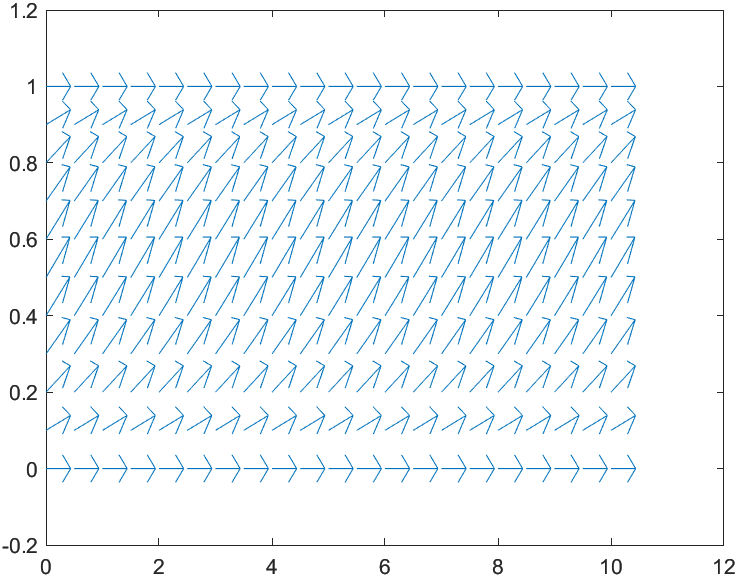
\includegraphics[height=\figHeight]{\autonomousDir/autonomous.png}}
			
			\subfloat[\raggedright separable: ${ y' = f(x) y (1-y) }$ where ${ f(x) = 0.2x }$]{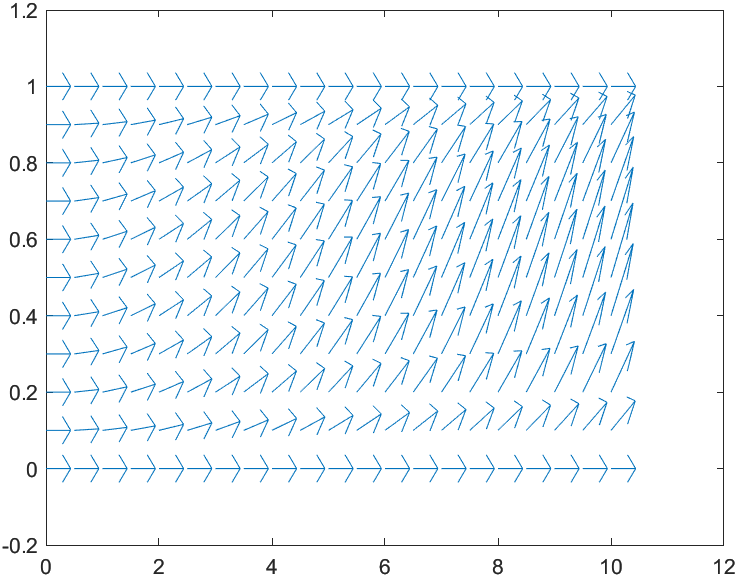
\includegraphics[height=\figHeight]{\autonomousDir/separable.png}}
			
			\subfloat[\raggedright non-separable: ${ y' = y (1-y) + f(x) }$ where ${ f(x) = 0.02x }$]{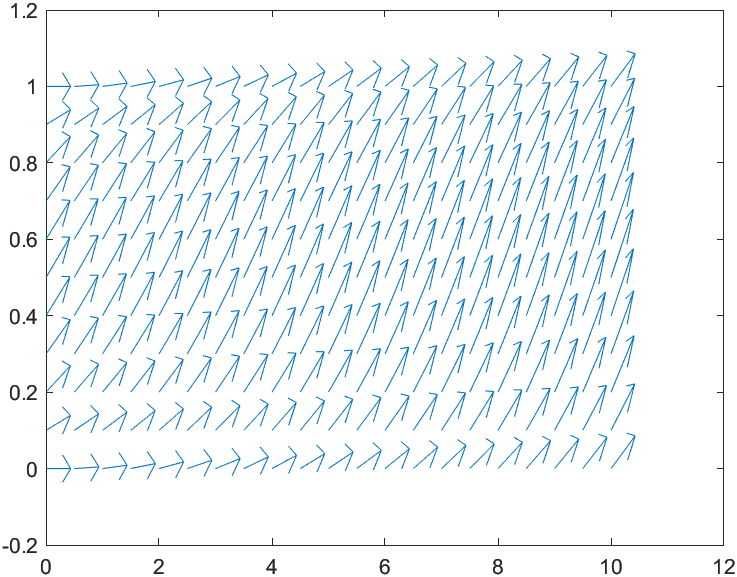
\includegraphics[height=\figHeight]{\autonomousDir/non_separable.png}}
			
			\caption{autonomous, separable and non-separable direction fields}%
		\end{figure}
		
		\boxeddefinition{An \textbf{exact} equation refers to a differential equation whose solutions all conserve the value of some property. All separable equations are exact equations because,
			\[ f(y) \dif y = g(x) \dif x \implies \int f(y) \dif y - \int g(x) \dif x = 0. \]
			However, there are also exact equations that are not separable such as,
			\[ y' \sin{x} + y \cos{x} + 2x = 0 \implies (y \sin{x} + x^2)' = 0 \implies y = \frac{C - x^2}{\sin{x}}. \]
		}
	
		\begin{tcolorbox}[breakable,enhanced jigsaw,colframe=white,colback=white,boxrule=0pt,arc=0pt,left=0pt,right=0pt,top=0pt,bottom=0pt]
			\labeledProposition{Let $y$ be any function satisfying the differential equation,
				\[ A(x,y) + B(x,y)\dod{y}{x} = 0 \]
				with
				\[ \dpd{A}{y} = \dpd{B}{x}. \]
				Then all such functions $y$ preserve some invariant property ${ \Psi(x,y) = C }$ for constant $C$.}{exact-equation-form-of-diff-eq}
			\begin{proof}
				The function $\Psi$ may consist of terms of only $x$, terms of only $y$, terms containing both $x$ and $y$ and a constant term. So we can describe it as,
				\[ \Psi(x,y) = p(x)q(y) + r(x) + s(y) + k \]
				where ${ p,q,r,s }$ are arbitrary functions and $k$ is a constant. But, since $\Psi$ will be a constant -- and we are only interested in the fact that it is constant, not the value of the constant -- we can ignore the constant term $k$ because it will just change the value of the constant that $\Psi$ is equal to. In other words, we can describe $\Psi$ as,
				\[ \Psi(x,y) = p(x)q(y) + r(x) + s(y) = C \]
				with $k$ absorbed into the value of $C$.\\
				
				Then, taking partial derivatives with respect to $x$ and $y$ we have,
				\[ \dpd{\Psi}{x} = \dod{p}{x} q(y) + \dod{r}{x} \eqand \dpd{\Psi}{y} = p(x) \dod{q}{y} + \dod{s}{y}. \]
				Furthermore, since $\Psi$ is a constant function we know that,
				\[ \dod{\Psi}{x} = 0 = \dpd{\Psi}{x} + \dpd{\Psi}{y} \dod{y}{x}. \]
				This has the required form ${ A(x,y) + B(x,y)\tod{y}{x} = 0 }$ with ${ \tpd{A}{y} = \tpd{B}{x} }$. So, if we have a differential equation of the given form and we postulate the existence of a constant function $\Psi$ such that ${ \tpd{\Psi}{x} = A(x,y) }$ and ${ \tpd{\Psi}{y} = B(x,y) }$, then,
				\begin{align*}
					\int A(x,y) \dif x = \int \dpd{\Psi}{x} \dif x &= \int \left( \dod{p}{x} q(y) + \dod{r}{x} \right) \dif x\nn
					 &= p(x) q(y) + r(x) + C_1(y), \nn
					\int B(x,y) \dif y = \int \dpd{\Psi}{y} \dif y &= \int \left( p(x) \dod{q}{y} + \dod{s}{y} \right) \dif y  \nn
					&= p(x) q(y) + s(y) + C_2(x).
				\end{align*}
				Comparing these two results,
				\[ \Psi(x,y) = p(x) q(y) + r(x) + C_1(y) = p(x) q(y) + s(y) + C_2(x), \]
				we can see that the function $\Psi(x,y)$ that we are looking for is ${ \Psi(x,y) = p(x)q(y) + r(x) + s(y) }$.\\
				
				Another way that we could have resolved $\Psi$ is to take the first integral,
				\[ \int A(x,y) \dif x = \int \dpd{\Psi}{x} \dif x = p(x) q(y) + r(x) + C_1(y) \]
				and say, if ${ \Psi(x,y) = p(x) q(y) + r(x) + C_1(y) }$ then,
				\[ \dpd{\Psi}{y} = p(x) \dod{q}{y} + \dod{C_1}{y} \]
				and compare this with ${ B(x,y) }$ to resolve the function $C_1$,
				\begin{align*}
					&& p(x) \dod{q}{y} + \dod{C_1}{y} &= B(x,y) = p(x) \dod{q}{y} + \dod{s}{y} \nn
					&\iff & \dod{C_1}{y} &= \dod{s}{y} \nn
					&\iff & C_1(y) &= s(y) + k &\sidecomment{integrating both sides wrt. $y$}
				\end{align*}
				where $k$ is a constant of integration which, in this case, can be ignored.
			\end{proof}
		\end{tcolorbox}
	
		\medskip
		\begin{tcolorbox}[breakable,enhanced jigsaw,colframe=white,colback=white,boxrule=0pt,arc=0pt,left=0pt,right=0pt,top=0pt,bottom=0pt]
			\labeledProposition{All separable equations are exact equations.}{separable-diff-eqs-are-exact}
			\begin{proof}
				A separable differential equation is one that may be put in the form,
				\[ f(y) \dif y = g(x) \dif x. \]
				We can re-arrange this,
				\begin{align*}
					&& f(y) \dif y &= g(x) \dif x \\
					&\iff & f(y) \dod{y}{x} - g(x) &= 0.
				\end{align*}
				Now, taking ${ A(x,y) = -g(x) }$ and ${ B(x,y) = f(y) }$ we have the form ${ A(x,y) + B(x,y) \tod{y}{x} = 0 }$ with ${ \tpd{A}{y} = \tpd{B}{x} = 0 }$ so this is an exact equation.
			\end{proof}
		\end{tcolorbox}
		
		
		
		\biggerskip\biggerskip
		\note{All autonomous equations are separable (though the reverse is not generally true) and all separable equations are exact equations (although some exact equations are not separable). So we have,
			\[ \{\text{Autonomous}\} \subset \{\text{Separable}\} \subset \{\text{Exact}\}. \]
		}
		
		
		\biggerskip
		\subsubsubsection{Examples of Exact Equations}
		\begin{exe}
			\item{Suppose we have the equation
				\[ (3x^2 + 2xy) + (2y + x^2)\dod{y}{x} = 0. \]
				We have,
				\[ \dpd{(3x^2 + 2xy)}{y} = 2x = \dpd{(2y + x^2)}{x} \]
				so this is an exact equation. We can solve for the constant function preserved by all solutions by setting
				\begin{align*}
					&& \int 3x^2 + 2xy \dif x &= \int 2y + x^2 \dif y \nn
					&\iff & x^3 + x^2y + C_1(y) &= y^2 + x^2y + C_2(x) &\sidecomment{} \nn
					&\iff & x^3 + C_1(y) &= y^2 + C_2(x) \nn
					&\therefore & \Psi(x,y) &= x^2y + y^2 + x^3 = C  &\sidecomment{for constant C}.
				\end{align*}
				So, all solutions $y(x)$ of this differential equation preserve the value of $\Psi$ and so, if we have an initial condition -- say ${ y(0) = 1 }$ -- then we can use this to find the value of ${ C = \Psi(0,1) }$ and this value will be preserved for all values of $x$ and $y$.
				\[ \Psi(0,1) = (0^2)(1) + (1)^2 + (0^3) = 1 = x^2y + y^2 + x^3 \hspace{20pt} \forall x,y \in \R{}. \]
				Now we can solve for $y$ by treating $x$ as a constant and arranging the equation as a quadratic in $y$:
				\[ y^2 + x^2 y + (x^3 - 1) = 0 \]
				and then using the quadratic formula for $y$,
				\[ y = \frac{-b \pm \sqrt{b^2 - 4ac}}{2a} = \frac{-x^2 \pm \sqrt{x^4 - 4x^3 - 4}}{2}. \]
			}
			\bigskip
			\item{Suppose we have the equation
				\[ (3x + 2y) + (\frac{2y}{x} + x)\dod{y}{x} = 0. \]
				This is equation is \textit{not} exact because,
				\[ \dpd{(3x + 2y)}{y} = 2  \neq \dpd{(\frac{2y}{x} + x)}{x} = \frac{-2y}{x^2} + 1. \]
				However, if we multiply the equation by $x$ then we get the equation in the previous example,
				\[ x(3x + 2y) + x(\frac{2y}{x} + x)\dod{y}{x} = (3x^2 + 2xy) + (2y + x^2)\dod{y}{x} = 0. \]
				So there are times when multiplying by an integrating factor can result in an exact equation.
			}
			\bigskip
			\item{
				Consider a body falling toward earth from a significant distance so that the change in acceleration due to gravity as the body gets closer to the earth is significant. Acceleration due to gravity is proportional to ${ 1/r^2 }$ where $r$ is the distance of the body from the centre of the earth -- remember the mass of the body is a multiplier of the force of gravity but also of the inertia so in the expression for the resultant acceleration the mass cancels out -- so we can model this situation as,
				\[ \dod[2]{r}{t} = -\frac{c}{r^2} \]
				where $c$ is a positive constant. Note that the expression on the right hand side is negative because $r$ is always positive but, in the scenario, is decreasing so ${ \tod{r}{t} }$ is negative, and it is getting more negative as $r$ gets smaller, so the second derivative is also negative.\\
				
				If we use classical Newtonian mechanics then we can model $r$ as a displacement $s$ from the center of the earth. Then the velocity ${ v = \tod{s}{t} }$ is negative as the body is falling towards the earth. We also have,
				\[ a = \dod[2]{s}{t} = \dod{v}{t} = \dod{v}{s} \cdot \dod{s}{t} = \dod{v}{s} \cdot v. \]
				Interestingly, we can see that,
				\[ \dod{v}{s} = \frac{a}{v} = \frac{\dif v/\dif t}{v} \]
				which is the log-derivative of $v$ representing the relative infinitesimal change (\href{https://en.wikipedia.org/wiki/Logarithmic_derivative}{wikipedia}) of the velocity and also,
				\[ \dod{v}{s} = \dod{(\dif s/\dif t)}{s} \]
				the way that the rate of change of the displacement changes with the displacement.\\
				
				If we consider the first-order equation
				\[ \dod{v}{s} v = -\frac{c}{s^2}, \]
				this has the form ${ y \tod{y}{t} = f(t) }$ and so, is separable. 
				\begin{align*}
					&& \dod{v}{s} v &= -\frac{c}{s^2} \\
					&\iff & \int v \dif v &= -c \int \frac{1}{s^2} \dif s &\sidecomment{} \nn
					&\iff & \frac{v^2}{2} &= -c \left(\frac{-1}{s}\right) + C &\sidecomment{} \nn
					&\iff & \frac{v^2}{2} &= \frac{c}{s} + C &\sidecomment{} \nn
					&\iff & \frac{v^2}{2} - \frac{c}{s} &= C.
				\end{align*}
				So the quantity ${ \frac{v^2}{2} - \frac{c}{s} }$ is preserved by all solutions of this differential equation. The gravitational potential energy of a body displaced from the earth is given (by Newton's 3rd law) as the work done if the body were to fall all the way to the earth's centre,
				\[ E_p = F \cdot s = m\, a(s)\, \cdot s \]
				where $m$ is the mass of the body, $s$ is the displacement of the body from the centre of the earth and $a$ is the acceleration due to gravity as a function of the displacement. Substituting in the function for the acceleration due to gravity as a function of the distance from the earth's centre we have,
				\[ E_p = m \left(-\frac{c}{s^2}\right) s = - \frac{mc}{s}. \]
				The kinetic energy of the falling body is given by,
				\[ E_k = \frac{mv^2}{2}. \]
				Since the falling movement of the body is the potential energy turning to kinetic energy, the sum ${ E_p + E_k }$ is conserved. So, for some constant $K$ we have,
				\begin{align*}
					&& \frac{mv^2}{2} - \frac{mc}{s} &= K \nn
					&\iff & m \left( \frac{v^2}{2} - \frac{c}{s} \right) &= K &\sidecomment{} \nn
					&\iff & \frac{v^2}{2} - \frac{c}{s} &= C &\sidecomment{for ${ C = K/m }$.} \\
				\end{align*}
			}
			\biggerskip
			\item{
				Imagine a pendulum swinging on a rod (or a rope that remains taut) of length $L$. Let $\theta$ be the angle the rod makes with the vertical and $g$ the acceleration due to gravity. The gravitational force acting on the pendulum has a component that is balanced by the tension in the rod maintaining the pendulum swinging along the circumference of a circle. This component acts in a direction perpendicular to the circumference of the circle in which the pendulum mass moves and along the radius of the circle of movement. The other component of $g$, orthogonal to this one, acts along the tangent of the circumference of movement of the pendulum mass. It is this component that creates the motion of the pendulum mass. (If this is not clear: \href{https://www.acs.psu.edu/drussell/Demos/Pendulum/Pendulum.html}{Penn State page on pendulum oscillation}.)\\
				
				We have:
				\begin{itemize}
					\item{Acceleration due to gravity with a component perpendicular to the pendulum rod given by: ${ a = - g \sin\theta }$.}
					\item{Angular velocity of the pendulum mass: ${ \omega = \dod{\theta}{t} }$.}
					\item{Tangential velocity of the pendulum mass: ${ v_t = L \dod{\theta}{t} }$.}
				\end{itemize}
				
				So, using ${ F = m\od{v}{t} }$, the equation describing the acceleration of the pendulum mass is,
				\begin{align*}
					&& m\dod{v_t}{t} &= - m g \sin\theta \nn
					&\iff & \dod{v_t}{t} &= - g \sin\theta &\sidecomment{} \nn
					&\iff &  L \dod[2]{\theta}{t} &= - g \sin\theta.
				\end{align*}
				
				This is a second-order nonlinear equation. For small oscillations we can use the small-angle approximation of sine to linearize it (see example \ref{ex:pendulum-second-order-linear}). If the oscillations are not small though, the small-angle approximation becomes too inaccurate to be useful and we must solve the nonlinear equation.\\
				
				We can simplify it into a first-order nonlinear equation by describing the tangential velocity in relation to the angle $\theta$ and eliminating time from the model,
				\[ v = L\omega = L\dod{\theta}{t} \iff \dod{\theta}{t} = \frac{v}{L}, \]
				\[ L \od[2]{\theta}{t} = \dod{v}{t} = \dod{v}{\theta} \cdot \dod{\theta}{t} = \dod{v}{\theta} \cdot \frac{v}{L} = - g \sin\theta. \]
				
				\bigskip
				So we end up with the \textit{separable} first-order nonlinear equation,
				\begin{align*}
					&& v \, \dod{v}{\theta} &= - gL \sin\theta \nn
					&\iff & \int v \dif v &= -gL \int \sin\theta \dif \theta &\sidecomment{} \nn
					&\iff & v^2 &= 2gL \cos\theta + C &\sidecomment{} \nn
					&\iff & v(\theta) &= \pm \sqrt{2gL \cos\theta + C}. \\
				\end{align*}
				Note that we have ended up with an expression for the tangential velocity as a function of the angle $\theta$ \textit{only}.  Also worth noting is that the constant quantity,
					\[ v^2 - 2gL \cos\theta = C \]
				represents the conserved energy of the pendulum system -- the $v^2$ term being proportional to the kinetic energy and the $2gL \cos\theta$ term being proportional to the potential energy.\\
				
				If we consider an oscillation with maximum angle $\theta_{max}$ then the pendulum is momentarily at rest when ${ \theta = \theta_{max} }$. It is convenient to use this as the initial condition of the angle of the pendulum ${ \theta_0 = \theta_{max} }$ so that the pendulum begins at rest and so ${ v(\theta_0) = 0 }$ and then we can resolve the value of the constant,
				\begin{align*}
					&& v(\theta_0) &= \pm \sqrt{2gL \cos\theta_0 + C} = 0 \\
					&\therefore & C &= - 2gL \cos\theta_0.
				\end{align*}
			
				So, for the initial condition,  we have resolved the tangential velocity \wrt to the angle of displacement of the pendulum as,
				\[ v(\theta) = \pm \sqrt{2gL (\cos\theta - \cos\theta_0)}. \]
				We could also have obtained this result with definite integration from $\theta_0$ to $\theta$,
				\begin{align*}
					&& \int_{v(\theta_0)}^{v(\theta)} v \dif v &= -gL \int_{\theta_0}^\theta \sin t \dif t \nn
					&\iff & \frac{1}{2} (v(\theta)^2 - v(\theta_0)^2) &= gL (\cos\theta - \cos\theta_0) &\sidecomment{} \nn
					&\iff & v(\theta)^2 &= 2gL (\cos\theta - \cos\theta_0) &\sidecomment{${ \because v(\theta_0) = 0 }$}. \\
				\end{align*}
			
				To recover the time information into the solution we can bring back the definition of the velocity as a function of time \textit{as well as} the angle of displacement,
				\[ v = L\dod{\theta}{t}. \]
				Substituting this back into the solution we get,
				\begin{align*}
					&& L\dod{\theta}{t} &= \pm \sqrt{2gL (\cos\theta - \cos\theta_0)} \\
					&\iff & \dif t &= \sqrt{\frac{L}{2g}} \frac{1}{\sqrt{\cos\theta - \cos\theta_0}} \dif \theta. &\sidecomment{}
				\end{align*}
			
				So, to find the time taken when the pendulum swings from its central position, with ${ \theta = 0 }$, to its amplitude, with ${ \theta_{max} = \theta_0 }$, we can integrate the expression on the right of this equation between $\theta_0$ and 0. To get the whole time period of the oscillation we can multiply this time by 4,
				\[ T = 4 \sqrt{\frac{L}{2g}} \int_{\theta_0}^0 \frac{1}{\sqrt{\cos\theta - \cos\theta_0}}  \dif \theta. \]
				This integral is a type of improper integral called an elliptic integral and it doesn't have an analytic solution. However, for small-angle oscillations we can use the small-angle approximation for cosine, 
				\[ \cos{x} = 1 - \frac{x^2}{2}, \]
				to obtain an approximate value of the integral,
				\begin{align*}
					&\int_{\theta_0}^0 \frac{1}{\sqrt{(1 - \frac{\theta^2}{2}) - (1 - \frac{\theta_0^2}{2})}}  \dif \theta  \nnn
					= &\int_{\theta_0}^0 \frac{1}{\sqrt{\frac{1}{2}(\theta_0^2 - \theta^2)}}  \dif \theta  \nnn
					= &\sqrt{2} \int_{\theta_0}^0 \frac{1}{\sqrt{\theta_0^2 - \theta^2}}  \dif \theta  \nnn
					= &\frac{\sqrt{2}}{\theta_0} \int_{\theta_0}^0 \frac{1}{ \sqrt{ 1 - \left(\frac{\theta}{\theta_0}\right)^2 } }  \dif \theta  \nnn
					= &\frac{\sqrt{2}}{\theta_0} \int_{\theta_0}^0 \frac{1}{ \sqrt{ 1 - \sin^2\alpha } }  \dif\, (\theta_0\sin\alpha)  \\[9pt]
					= &\frac{\sqrt{2}}{\theta_0} \int_{\inv\sin(1)}^{\inv\sin(0)} \frac{\theta_0\cos\alpha}{\cos\alpha}  \dif \alpha  \\[9pt]
					= &\sqrt{2} (\inv\sin(0) - \inv\sin(1))  \nnn
					= &\sqrt{2} \left( - \frac{\pi}{2} \right) = - \frac{\pi}{\sqrt{2}}.  \\
				\end{align*}
				In this case we can ignore the minus sign -- it's merely a factor of the choice that $\inv\sin$ has to make in order to be a function; returning $\frac{\pi}{2}$ for $\inv\sin(1)$ instead of $- \frac{\pi}{2}$. So, the time period becomes,
				\[ T = 4 \sqrt{\frac{L}{2g}} \left( \frac{\pi}{\sqrt{2}} \right) = 2\pi \sqrt{\frac{L}{g}}. \]
				Note that the amplitude of the pendulum's oscillation $\theta_0$ cancelled out in the calculation of the time period and that the resultant expression for the \textit{time period of small oscillations} of a pendulum depends only on the length of the string and the acceleration due to gravity.
			}\label{ex:pendulum-first-order-exact}
		\end{exe}
		
		\biggerskip\sep\biggerskip
		\parbox{\linewidth}{
			\subsubsubsection{Homogeneous Differential Equations}
			\boxeddefinition{A \textbf{homogeneous differential equation} is an equation of the form,
				\[ f(x,y)\frac{\dif y}{\dif x} = g(x,y) \]
				where the functions $f,g$ are both homogeneous of degree $d$.
			}
		}
		
		\bigskip\note{The functions $f,g$ need not be linear and so these differential equations are not necessarily linear.}
		
		The key insight here is that, due to the homogeneous function property (see: \ref{section:homogeneous-functions}), if we define the function $y$ to be ${ y(x) = x \cdot v(x) }$ --- which we may do because, due to the non-trivial kernel of differentiation, we are only able to determine a solution to a differential equation upto a constant term so we can set the constant term to 0 for convenience during the calculation --- then,
		\[ f(\lambda x, \lambda y) = \lambda^d f(x,y) \implies f(x,xv) = x^d g(v). \]
		When this is applied in a differential equation of the above form we obtain,
		\begin{align*}
			&& f(x,y)\frac{\dif y}{\dif x} &= g(x,y) \\[8pt]
			&\iff & x^d f_1(v) \left(v + x\frac{\dif v}{\dif x}\right) &= x^d f_2(v) &\sidecomment{${y = xv,\,\, y' = v + xv'}$} \\[8pt]
			&\iff & f_1(v) \left(v + x\frac{\dif v}{\dif x}\right) &= f_2(v) &\sidecomment{} \\[8pt]
			&\iff & v + x\frac{\dif v}{\dif x} &= \frac{f_2(v)}{f_1(v)} = f_3(v) &\sidecomment{} \\[8pt]
			&\iff & x\frac{\dif v}{\dif x} &= f_3(v) - v = f_4(v) &\sidecomment{} \\[8pt]
			&\iff & \frac{1}{f_4(v)}\frac{\dif v}{\dif x} &= \frac{1}{x} &\sidecomment{} \\[8pt]
			&\iff & \int \frac{1}{f_4(v)}\frac{\dif v}{\dif x} \dif x &= \int \frac{1}{x} \dif x = \ln{\abs{x}} + c &\sidecomment{} \\[8pt]
			&\iff & \int \frac{1}{f_4(v)} \dif v &= \ln{\abs{x}} + c &\sidecomment{} \\[8pt]
			&\iff & \frac{1}{f_4'(v)} \ln{\abs{f_4(v)}} &= \ln{\abs{x}} + c. &\sidecomment{} \\[8pt]
		\end{align*}
	}




% ---------------- break --------------

	\pagebreak
	\searchableSubsection{Comparison of Differential Equations with Difference Equations}{differential equations}{
		\TODO{Comparison of Differential Equations with Difference Equations}
	}
% ------------------

	\pagebreak
	\searchableSubsection{Second-order Linear ODEs}{differential equations}{
		
		\subsubsection{Examples of Second-order Linear}
		\begin{exe}
			\ex{\textbf{The Logistic:} The logistic model of population growth takes $P(t)$ to be the population at time $t$. The model takes some additional factor that illustrates that a space can only hold a fixed carrying capacity of the population, producing the equation
				\[ \frac{\dif P}{\dif t} = c P(t) \left( 1 - \frac{P(t)}{A} \right). \]
				
				\subsubsubsection{From looking at the differential equation}
				Whatever the value of the derivative, we can see that the scalar $c$ will increase its magnitude thereby amplifying changes. So, $c$ is the growth rate and larger values of $c$ cause the population to change more rapidly.\\
				
				The steady-states of $P(t)$ are at the values such that the derivative is 0. Therefore,
				\[  c P(t) \left( 1 - \frac{P(t)}{A} \right) = 0 \implies P(t) \in \{0,1\}. \]
				Looking at the steady-states one-by-one:
				\begin{itemize}
					\item{$\bm{ P(t) = 0 }$: If $P(t)$ climbs above 0 then the derivative will be positive and so the function will be increasing away from the steady-state at 0. This is therefore an \textit{unstable} steady-state.
						\note{Note that, since $P(t)$ is a population, negative values don't make sense.}
					}
					\item{$\bm{ P(t) = A }$: If $P(t)$ is less than $A$ then the derivative will be positive and so the function will be increasing toward the steady-state at A. This is therefore a \textit{stable} steady-state from below. Also, if $P(t)$ is greater than $A$, the derivative is negative and so the function is decreasing towards the steady-state value at $A$ -- so this a \textit{stable} steady-state from above also. However, if the initial population value is less than $A$, then the population will never arrive at values above $A$ and this is the way that this function is normally used -- taking values between 0 and $A$. From either side, the larger the value of the growth rate $c$, the faster the function will approach the steady-state.
					}
				\end{itemize}
				
				\bigskip
				\subsubsubsection{Finding the solution}
				The equation is separable so we have,
				\begin{align*}
					&& \frac{\dif P}{\dif t} &= c P \left( 1 - \frac{P}{A} \right) \\[6pt]
					&\iff & \frac{\dif P}{\dif t} &= \left(\frac{c}{A}\right) P ( A - P) &\sidecomment{} \\[6pt]
					&\iff & \frac{1}{P ( A - P)} \dif P &= \left(\frac{c}{A}\right) \dif t  &\sidecomment{} \\[6pt]
					&\iff & \int \frac{1}{AP} + \frac{1}{A(A - P)} \dif P &= \int \left(\frac{c}{A}\right) \dif t  &\sidecomment{by partial fractions} \\[6pt]
					&\iff & \int \frac{1}{P} + \frac{1}{(A - P)} \dif P &= \int c \dif t  &\sidecomment{by partial fractions} \\[6pt]
					&\iff & \ln{P} - \ln{(A-P)} &= c t + D  &\sidecomment{$D$ is const. of integration} \\[6pt]
					&\iff & \ln{\left(\frac{P}{A-P}\right)} &= c t + D  &\sidecomment{} \\[6pt]
					&\iff & \frac{P}{A-P} &= B e^{ct}  &\sidecomment{$B=e^D$} \\[6pt]
					&\iff & P &= B e^{ct} (A - P)  &\sidecomment{} \\[6pt]
					&\iff & P(1 + B e^{ct}) &= AB e^{ct}  &\sidecomment{} \\[6pt]
					&\iff & P &= A \left( \frac{B e^{ct}}{1 + B e^{ct}} \right).
				\end{align*}
				\note{Note that:
					\begin{itemize}
						\item{Another common way to write the logistic function is to divide by ${  B e^{ct} }$ to get:
							\[ A \left( \frac{1}{E e^{-ct} + 1} \right) \]
							where ${ E = \frac{1}{B} }$.
						}
						\item{As has been noted: ${ 0 \leq P(t) \leq A }$. So,
							\begin{align*}
								&& 0 \leq  A &\left( \frac{B e^{ct}}{1 + B e^{ct}} \right) \leq A \\
								&\iff & 0 \leq  &\left( \frac{B e^{ct}}{1 + B e^{ct}} \right) \leq 1.  \\
							\end{align*}
							The value,
							\[ \frac{B e^{ct}}{1 + B e^{ct}} = \frac{1}{E e^{-ct} + 1} \]
							is a proportion, a value in ${ [0,1] }$.
						}
						\item{Since we have,
							\[ P(t) = A \theta \]
							where $\theta$ is a proportion and the derivative is given by,
							\[ \frac{\dif P(t)}{\dif t} = c A \theta (1 - \theta) = cA\theta - cA\theta^2 \]
							we can see that if $\theta$ is small then the derivative will be approximately,
							\[ cA\theta = cP(t). \]
							For this reason, when $\theta$ is small -- which happens when $t$ is small -- the growth of the function is approximately exponential.
						}
					\end{itemize}	 
				}
			}
			\biggerskip
			\ex{\textbf{Simple Harmonic Motion:} ${ y'' = -ky }$ \TODO{S.H.M.}}
			\biggerskip
			\ex{
				
				This is a second-order non-linear equation but, for small angular displacements, we can linearize this equation using the small-angle approximation for sine ${ \sin\theta \approx \theta }$ giving:
				\begin{align*}
					&&  L \od[2]{\theta}{t} &= - g \theta \\
					&\iff & \od[2]{\theta}{t} &= - \frac{g}{L} \theta &\sidecomment{} \\
					&\iff & \od[2]{\theta}{t} + \frac{g}{L} \theta &= 0.
				\end{align*}
				The auxiliary equation of this equation is ${ z^2 + \frac{g}{L} = 0 }$ -- the roots of which are clearly complex and given by,
				\[ z = \pm \frac{\sqrt{-4(g/L)}}{2} = \pm \sqrt{-\frac{g}{L}} = \pm \sqrt{\frac{g}{L}} i. \]
				
				\TODO{2nd order linearized pendulum equation}
				
			}\label{ex:pendulum-second-order-linear}
		\end{exe}
	}

% ------------------

	\pagebreak
	\searchableSubsection{Second-order Nonlinear ODEs}{differential equations}{
		\biggerskip
		
		\subsubsection{Examples of Second-order Nonlinear}
	}

\end{document}